\section{Experiment 1: Reducing Training Data With Care}

% Corresponding Progress Reports
% https://www.notion.so/241122-Matthias-first-exploration-for-image-dropout-ccb558156ba04efab6435b0f42021d44
% https://www.notion.so/241129-Matthias-Dropout-experiment-first-results-dac4111347ec413c87bbdfdaf4ef495e?pvs=23
% https://www.notion.so/241213-Matthias-ICNN-in-image-dropout-9e810b27443c400f902e232cf966004d?pvs=23
% https://www.notion.so/241220-Matthias-reducing-train-data-with-care-First-AI-captions-0a0a3c610dba4d9c84d4eda4fb1c53dd?pvs=23
% https://www.notion.so/20250117-Matthias-Filling-the-gaps-1-7126a49b2ee34921aff7e853c3a1542c?pvs=23
% https://www.notion.so/Matthias-Mildenberger-243a8aff9cee491a987bc227e5c937cc?p=ef08526d469548adbeedae4384177db1&pm=s
% https://www.notion.so/250214-matthias-filling-the-gaps-4-197726ec52d680a28b00db7958f00613?pvs=23

\subsection{Background}

This work will focus on how data diversity at different levels can affect the performance of image reconstruction from  brain activity. Since we cannot easily increase data diversity in our experimental setup, or at least it would require a lot of effort (recording new data takes time and money), we are trying to find ways to investigate how we can manipulate the data diversity  without recording new data. In this first experiment, we first take a backward approach: we reduce the training data in a guided way. The reduction is performed under different subsampling criteria, which relate to different aspects of data diversity. The aim is to find a way to reduce the training data that allows a reconstruction performance similar to (or even better than) the full data set. This will allow a first exploration of what aspects should be considered when creating a possible new data set, in order to achieve the best possible results in future new experiments where new brain activity can also be recorded. 

Many studies have explored how to achieve comparable results with reduced training data sets as with the full data set. Wang et al.\cite{wangDataDropoutOptimizing2018} used a two-step procedure, first training the model on the full training data and then using the validation data to delete any training samples that would reduce the overall loss on the validation data set. This allowed them to remove unfavourable training samples and end up training a new model on a reduced dataset, which actually performed better than the full dataset on the test data. Sener et al.\cite{senerActiveLearningConvolutional2018} were able to use a core set approach in active learning to ensure that the data selected during model training would yield the greatest improvement, thus achieving good classification even with greatly reduced datasets. They were able to outperform many other algorithms and a random subselection baseline. In a detailed review, Guo et al.\cite{guoDeepCoreComprehensiveLibrary2022} compared different approaches to core set selection, highlighting in particular that random subselection is still a very strong baseline, often outperforming many targeted core set approaches. In a dataset for medical imaging of the heart, Kolluru et al.\cite{kolluruLearningFewerImages2021} were able to reduce the data to almost a tenth of its original size and still achieve acceptable results. They first used an autoencoder to map the images into an abstract feature space, then used PCA to further reduce the dimensionality, and finally used the k-medoids algorithm to form as many clusters in the reduced space as there were images to be extracted from the dataset. In summary, targeted reduction of training data is a promising approach to achieving stable performance with significantly fewer resources during training (and presumably data collection). However, it is not trivial to find a way to reduce the data in such a way that a random baseline can be beaten.


% Viele Studien haben sich bisher der Forschung danach gewidment, wie man mit reduzierten Trainingsdatensätzen vergleichbare Ergebnisse wie mit dem vollen Datensatz erzielen kann. Wang et al.\cite{wangDataDropoutOptimizing2018} haben in einem zweistufigen Verfahren das model zunächst auf allen Trainingsdaten trainiert und dann mithilfe des Validation Datensatzes alle Trainingssamples gelöscht, welche dafür sorgten dass der gesamtloss auf dem Validation Dataset verringert würde. Dadurch konnten sie unfavorable Trainingssamples entfernen und mit dem reduzierten Datensatz am Ende ein neues model trainieren, was gegenüber dem vollen Datensatz sogar eine bessere Leistung erbracht hat. Sener et al.\cite{senerActiveLearningConvolutional2018} konnten mit einem core set approach beim active learning dafür sorgen, dass während des trainings des models jeweils die Daten ausgewählt wurden, welche das größte improvement erzeugen würden und damit gegenüber vielen anderen approaches und zufälliger Auswahl auch mit stark verringerten Datensätzen gute Klassifikation erzielen. In einem ausführlichen Review haben Guo et al.\cite{guoDeepCoreComprehensiveLibrary2022} verschiedene Ansätze für eine core set selection miteinander verglichen und dabei insbesonere auch herausgestellt, dass die random subselection nach wie vor eine sehr starke baseline ist, welche viele gezielte core-set approaches häufig in den Schatten stellt. In einem Datensatz für medizinische Bildgebung am Herzen konnten Kolluru et al.\cite{kolluruLearningFewerImages2021} die Daten auf fast ein Zehntel der ursprünglichen Größe reduzieren und weiterhin passable Ergebnisse erzielen. Hierzu haben sie zunächst mit einem autoencoder die Bilder in einen abstrakten Feature space gebracht, dann mit einer PCA die Dimensionalität weiter reduziert und schließlich mit dem k-medoids Algorithmus so viele Cluster in dem reduzierten space gebildet, wie Bilder aus dem Datensatz extrahiert werden sollen. Zusammenfassend lässt sich sagen, dass eine gezielte Reduktion von Trainingsdaten ein vielversprechender Ansatz ist, um mit bedeutend weniger Ressourcen beim Training (und mutmaßich bei der Datenerhebung) eine stabile Performance zu erzielen. Dabei ist es aber nicht trivial, einen Weg zu finden, die Daten so zu reduzieren, dass eine random baseline geschlagen werden kann.

% - Diese Arbeit soll sich mit der data diversity beschäftigen, schauen wie die Diversität auf verschiedenen Ebenen die Rekonstruktionsleistung beeinflussen kann

% - Da wir innerhalb unseres Versuchsaufbaus die Datendiversität nicht ohne weiteres erhöhen können wird zunächst versucht durch gezielte Reduktion der Menge an Trainingsdaten überprüft, wie Subsamples mit unterschiedlichen Sampling Criteria jeweils die Leistung beeinflussen können

% - Related Works zur Reduction
  % - \cite{wangDataDropoutOptimizing2018} Entfernen unfavorable examples beim Training und versuchen dadurch die Generalisierungsfähigkeit zu verbessern
    % - They do a loss based dropout. It is done in an iterative fashion by checking how the loss on the validation set would change by removing single samples. They were able to increase the performance on classification and denoising tasks. 
  % - \cite{senerActiveLearningConvolutional2018} Nutzen einen Core-Set approach um die Daten zu reduzieren
    % - Wollen damit rausfinden, welche Daten man am besten labeln soll, weil das ein teures unterfangen ist
    % - Machen das ganze beim active learning, also quasi während dem Training werden die samples gesucht und mithilfe der Distance der final layer während des Trainings werden die most meaningful samples gesucht
    % - So kann man bei gezielten Aussuchen während dem Trainingsprozess bessere subsamples mit gleicher Größe erzeugen
  % - \cite{guoDeepCoreComprehensiveLibrary2022} Coreset selection review
  %   - Vergleichen 12 verschiedene popular methods und haben sie in einer Library zusammengebracht
  %   - Random ist immernoch eine sehr starke baseline
  % - \cite{kolluruLearningFewerImages2021}
  %   - Haben die Datenreduktion auch auf einen medizinischen Kontext angewendet, in dem Bilder einer
  % - \cite{kolluruLearningFewerImages2021} Reducing Images and maintaining good performance can also be used in medical context 
    % - Images first with autoencoder in lower level space, then with PCA space even smaller and subselection, good performance with even 0.1 of training data
  % Grundsätzlich ist es also gut möglich das zu tun, auch wenn teilweise zufällige Auswahl von Bildern schon sehr gut ist und an manchen Stellen fraglich, ob man diese überhaupt großartig schlagen kann
    
The aim of the study should be to investigate how maximising the low-level diversity of images (colours, shapes, textures) differs from maximising the high-level diversity (semantic concepts). To do this, the images would first need to be clustered in relation to the different features in order to make an appropriate subselection. Simple low-level clustering could be achieved by using only the distribution of colours in an image for clustering\cite{maheshwariImageClusteringUsing2009}. More modern approaches use the activation of pre-trained deep learning models to embed images in a more abstract feature space, so that semantic clustering can be performed in this space\cite{chang2017deep}. Birdokar et al.\cite{birodkarSemanticRedundanciesImageClassification2019} use different feature layers of a CNN to perform image clustering at different levels (low, mid and high level features). The late layer was especially useful for extracting the semantic features of the images and clustering was used to remove redundant samples. To make clustering algorithms such as k-means computationally feasible, the data from the extracted features must be reduced in dimensionality at best, UMAP\cite{mcinnesUMAPUniformManifold2018} is a modern algorithm that can be used for this. To cluster the images in a low-level space, UMAP can also be applied directly to the images without first embedding them in a feature space. After dimensionality reduction, the subsampled datasets can then be generated by clustering in the different feature levels and using those clusters as the subsampled dataset.


% Ziel der Studie soll es sein, zu untersuchen, wie sich eine Maximierung der low-level Diversity der Bilder (Farben, Formen, Texturen) versus der high-level Diversity (semantische Konzepte) voneinander unterscheidet. Dazu müssten die Bilder zunächst im Bezug auf die verschiedenen Features geclustered werden, um eine enstprechede Subselection treffen zu können. Einfache low-level clusterings könnten erzielt werden, indem lediglich die Verteilung der Farben in einem Bild für das Clustering genutzt wird\cite{maheshwariImageClusteringUsing2009}. Modernere Ansätze benutzen die Aktivationen von vortrainierten Deep Learning Modellen um Bilder in einen abstrakteren Feature space einzubetten, sodass in diesem ein semantisches Clsutering vorgenommen werden kann\cite{chang2017deep}. Birdokar et al.\cite{birodkarSemanticRedundanciesImageClassification2019} nutzen unterschiedliche Feature Layer eines CNN um auf verschiedenen Ebenen ein Bildclustering vorzunehmen. Dabei konnten mithilfe der späten layer sehr gut die semantischen Features der Bilder extrahiert werden und durch clustering redundante Samples entfernt werden. Damit Clustering Algorithmen wie k-means rechnerisch durchführbar sind, müssen die Daten aus den extrahierten Features bestenfalls in ihrer Dimensionalität reduziert werden, UMAP\cite{mcinnesUMAPUniformManifold2018} ist ein moderner Algorithmus welcher dafür genutzt werden kann. Um die Bilder in einem low-level space zu clustern kann UMAP auch direkt auf die Bilder angewendet werden ohne sie davor in einen Feature Space einzubetten. Nach der Reduktion der Dimensionalität können dann in den unterschiedlichen Feature Ebenen durch clustering die Subsampled datasets erstellt werden.

With respect to decoding brain activity, it has been previously found that different levels of the visual system are also better at predicting different feature levels (i.e., low-level brain structures such as V1 and V2 are better at predicting low-level features, and high-level structures such as PPA and FFA are better at predicting high-level features)\cite{horikawaGenericDecodingSeen2017}. However, to the best of our knowledge, there has been no systematic investigation of how maximising the diversity of training data at different feature levels (low-level vs.\ high-level) affects the decoding of brain data and the subsequent reconstruction of images. In other words, whether it is more important to have a training set that contains as many different semantic concepts as possible, or to use a training set that contains as many different low-level features (e.g.\ colours and shapes) as possible. 


% Ziel soll es bei unser Method sein, dass wir verschiedene Feature Spaces wollen, 
%   - Wollen untersuchen ob die Diversity in high vs low level sich unterscheidet darin, wie die Rekonstruktionen funktionieren können
%   - Wir müssen also meaningful subselections innerhalb der unterschiedlichen Feature Spaces finden können. 
%   - Dazu müssen wir erstmal die Bilder clustern um innerhalb der feature spaces ähnliche Bilder voneinander zu trennen

% Arbeiten zum Clustering
% - \cite{maheshwariImageClusteringUsing2009} 
%   - Datensätze können geclustert werden und so ähnliche Bilder automatisch gefunden werden
%   - Dies kann aufgrund von einfachen features wie Farben getan weren
% - \cite{chang2017deep}
%   - Clustering mithilfe von Aktivationen in einem CNN (sodass nur der letzte Feature Vector benutzt wird) können abstraktere Cluster ermöglichen
% - \cite{birodkarSemanticRedundanciesImageClassification2019}
%   - Finden semantisch redundante Bilder in öffentlichen Datensätzen
%   - Nutzen dafür anfängliche, mittlere und späte layer in resnets
%   - mit den späten layern konnte die semantische Redundanz am besten verringert werden
% - \cite{mcinnesUMAPUniformManifold2018}
  % - Mit Dimensionality Reduction methods können clusterings in geringeren Dimensionen erstellt werden, dies kann sowohl auf den image space (sodass nur die puren Pixel Informationen genutzt werden) angewandt werden oder auf beliebige Feature spaces welche das Augenmerk auf höherwertige semantische Kategorien legen

% In unserem Wissen wurde bisher noch keine systematische Untersuchung durchgeführt, welche die Diversität auf verschiedenen Bild Ebenen (low-level vs high level) untersucht und miteinander vergleicht. Insebsondere gibt es noch keine Forschung dazu, wie anhand von solchen Kriterien ausgewählte subspaces beim brain-decoding genutzt werden.

Our hypothesis is that the feature level at which the diversity of the training data is maximised will have a congruent effect on the performance on the test data. In particular, the decoding and reconstruction of artificial shapes should benefit from a focus on low-level feature diversity (since these have low semantic meaning). A focus on high-level diversity should improve performance on the natural test data (since the translator must be able to predict the semantic concepts of the images to properly reflect the test data). Furthermore, it is hypothesised that a focus on mid-level features (i.e.\ both low-level and high-level features) can provide the best overall performance on both test datasets. The baseline for all experiments should be random subselections to see if the diversity based subselections are actually able to have a real effect.

% Hypothesen:
% - Low-level Sampling soll low-level Algorithmen VDVAE und ICNN verbessern
%   - Insbesondere auch bei den artificial Shapes
% - Mid-Level Sampling mit dreamsim sollte die besten Ergebnisse produzieren, da sowohl auf gleichmäßige Verteilung der low als auch high level features geachtet wird
% - Mit high-level Sampling bestenfalls clip translator und die clip-accuracy bei der reconstruction


\subsection{Methods}

The procedure for obtaining a reduced training data set with maximised diversity is described below.

\subsubsection{Baseline with random dropout}

In order to evaluate diversity-based methods, it is important to establish a suitable baseline against which the results can be compared. To this end, reconstruction is first performed on a randomly subsampled training set. To get a better idea of the size of the training set needed to train the decoders, different data fractions are used. The full training set consists of 1200 images (and the corresponding recorded MRI activity). For the baseline, 10\% (120 images), 25\% (300 images), 50\% (600 images), 75\% (900 images) and 100\% of the images are used to train the decoder. This baseline is only performed for one subject (S2) to save computational resources. To control the sampling error, 5 random samples are taken for each data fraction and used to train the decoders. If all training images are used, only one sample can be taken (the full data set). 

% 1. Decoder Random Plot test/art

\begin{figure}[ht]
    \centering
    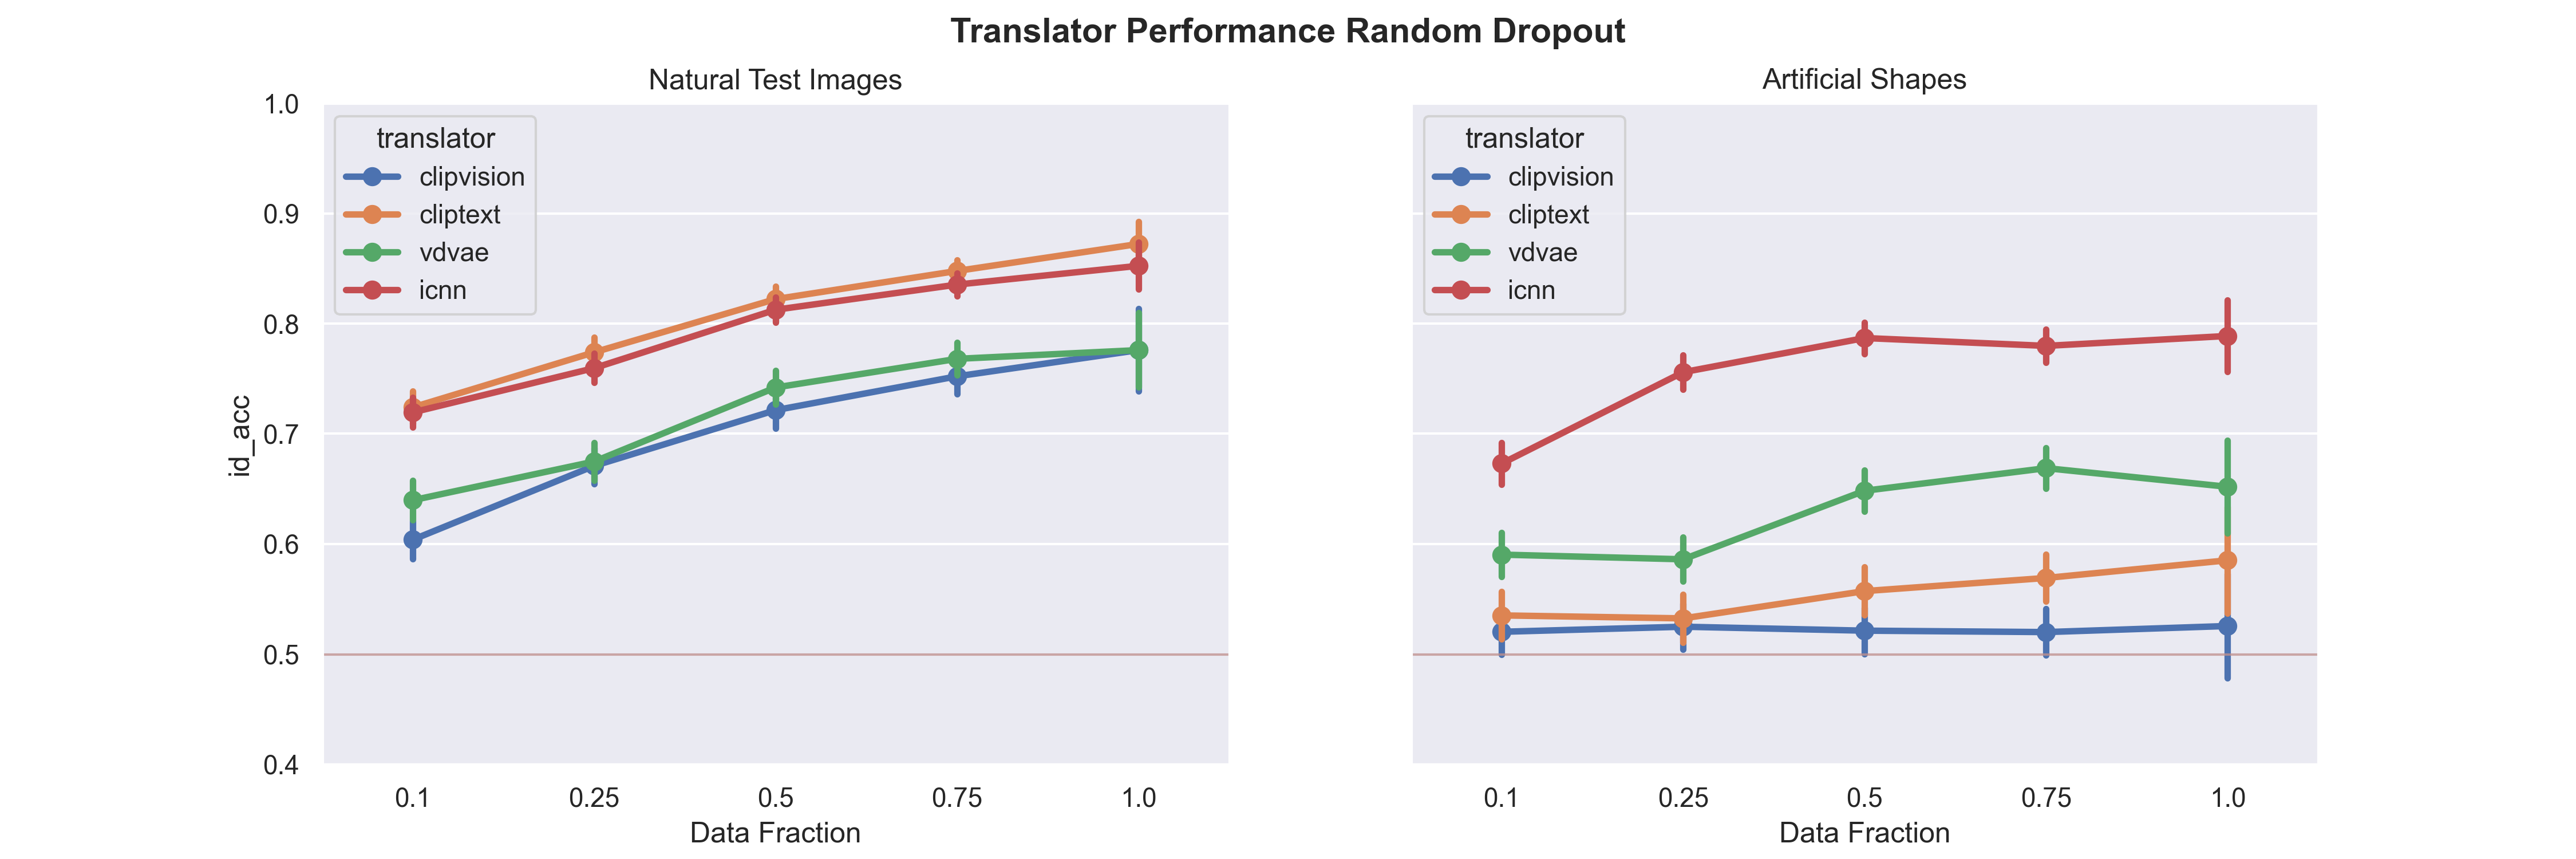
\includegraphics[width=1\textwidth]{plots/dropout_random_translator.png}
    \caption{Decoder Performance with different levels of random dropout}\label{fig:dropout_random_translator}
\end{figure}

% 2. Reconstruction Random Quant Plot test/art
\begin{figure}[ht]
    \centering
    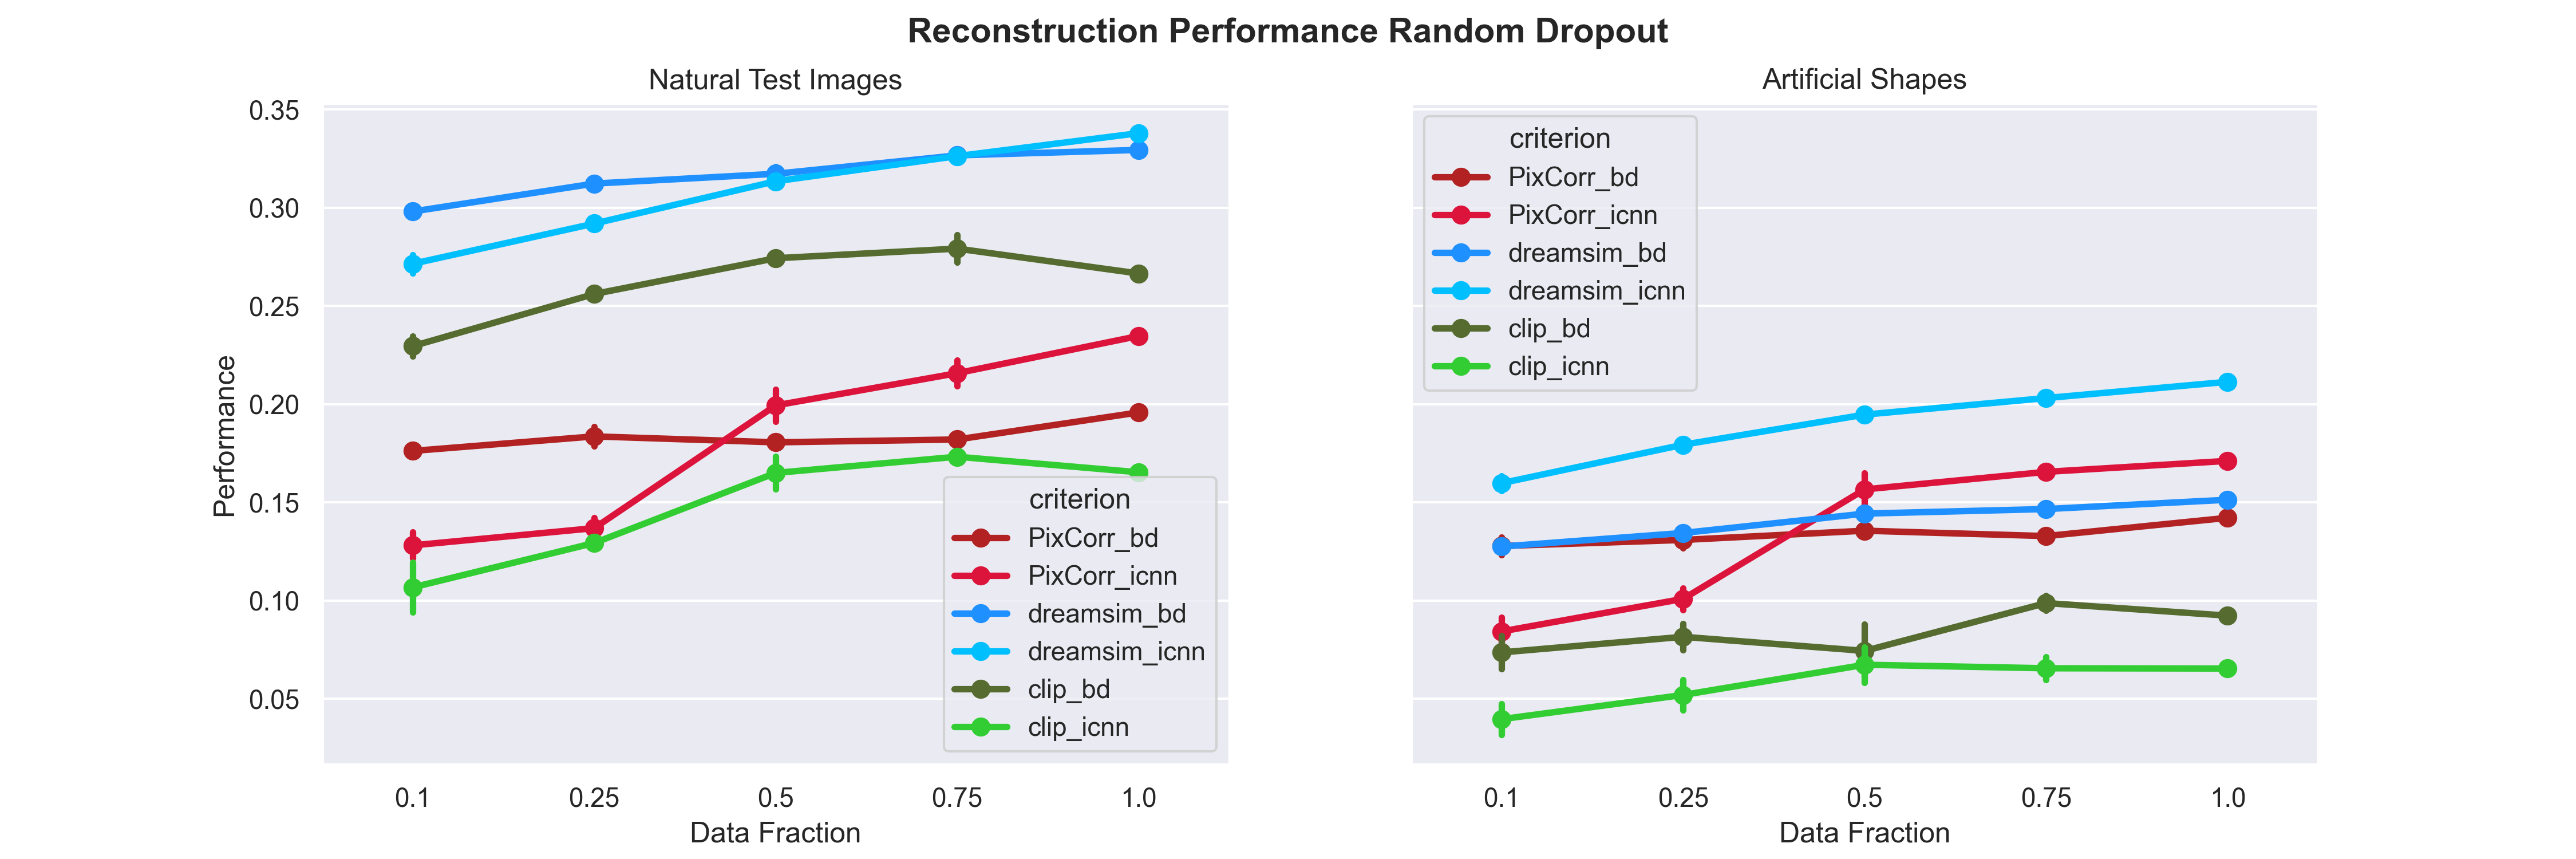
\includegraphics[width=1\textwidth]{plots/dropout_random_reconstruction.png}
    \caption{Reconstruction performance with different levels of random dropout}\label{fig:dropout_random_reconstruction}
\end{figure}

The performance of the translator is shown in Figure~\ref{fig:dropout_random_translator} for both the natural test images and the artificial shapes. For the natural test images, the relationship between the number of training samples and performance is relatively similar for all the translators: the more training samples, the better. However, for the VDVAE and ICNN in particular, the performance curve for the translator flattens out at around 50\% training samples. The trend for the artificial shapes is somewhat different. The Clipvision translator does not seem to improve with an increasing number of training images, but is only just above the random level of 0.5. The Cliptext translator can show a performance above the random level from about 50\% of the training data set and then increases continuously. The VDVAE translator shows a slightly higher performance, but also saturates at about 50\% of the training data set. The same pattern is shown by the ICNN, whose performance is the best, but also does not improve from about 50\% of the training data set. 

The quantitative performance of the reconstruction algorithms is shown in Figure~\ref{fig:dropout_random_reconstruction} for both the natural test images and the artificial images. The individual metrics are shown in similar colours for Brain Diffuser and ICNN (ICNN is slightly lighter than Brain Diffuser). The PixelCorrelation shows a similar picture for both algorithms for the natural test images and the artificial shapes: While the ICNN benefits from more training samples, with the step from 25\% to 50\% of the training data set being particularly significant, the brain-diffuser shows only a very small increase in performance with increasing number of training samples. The Dreamsim similarity increases continuously with a larger number of training samples. In particular, the ICNN benefits from a larger number of training samples. The Clip-Accuracy shows that for the natural test images the performance also saturates at about 50\% of the training samples, and for the artificial shapes it is difficult to report an increase in performance.

% 3. Reconstruction Random Qual Plot test

\begin{figure}[ht]
    \centering
    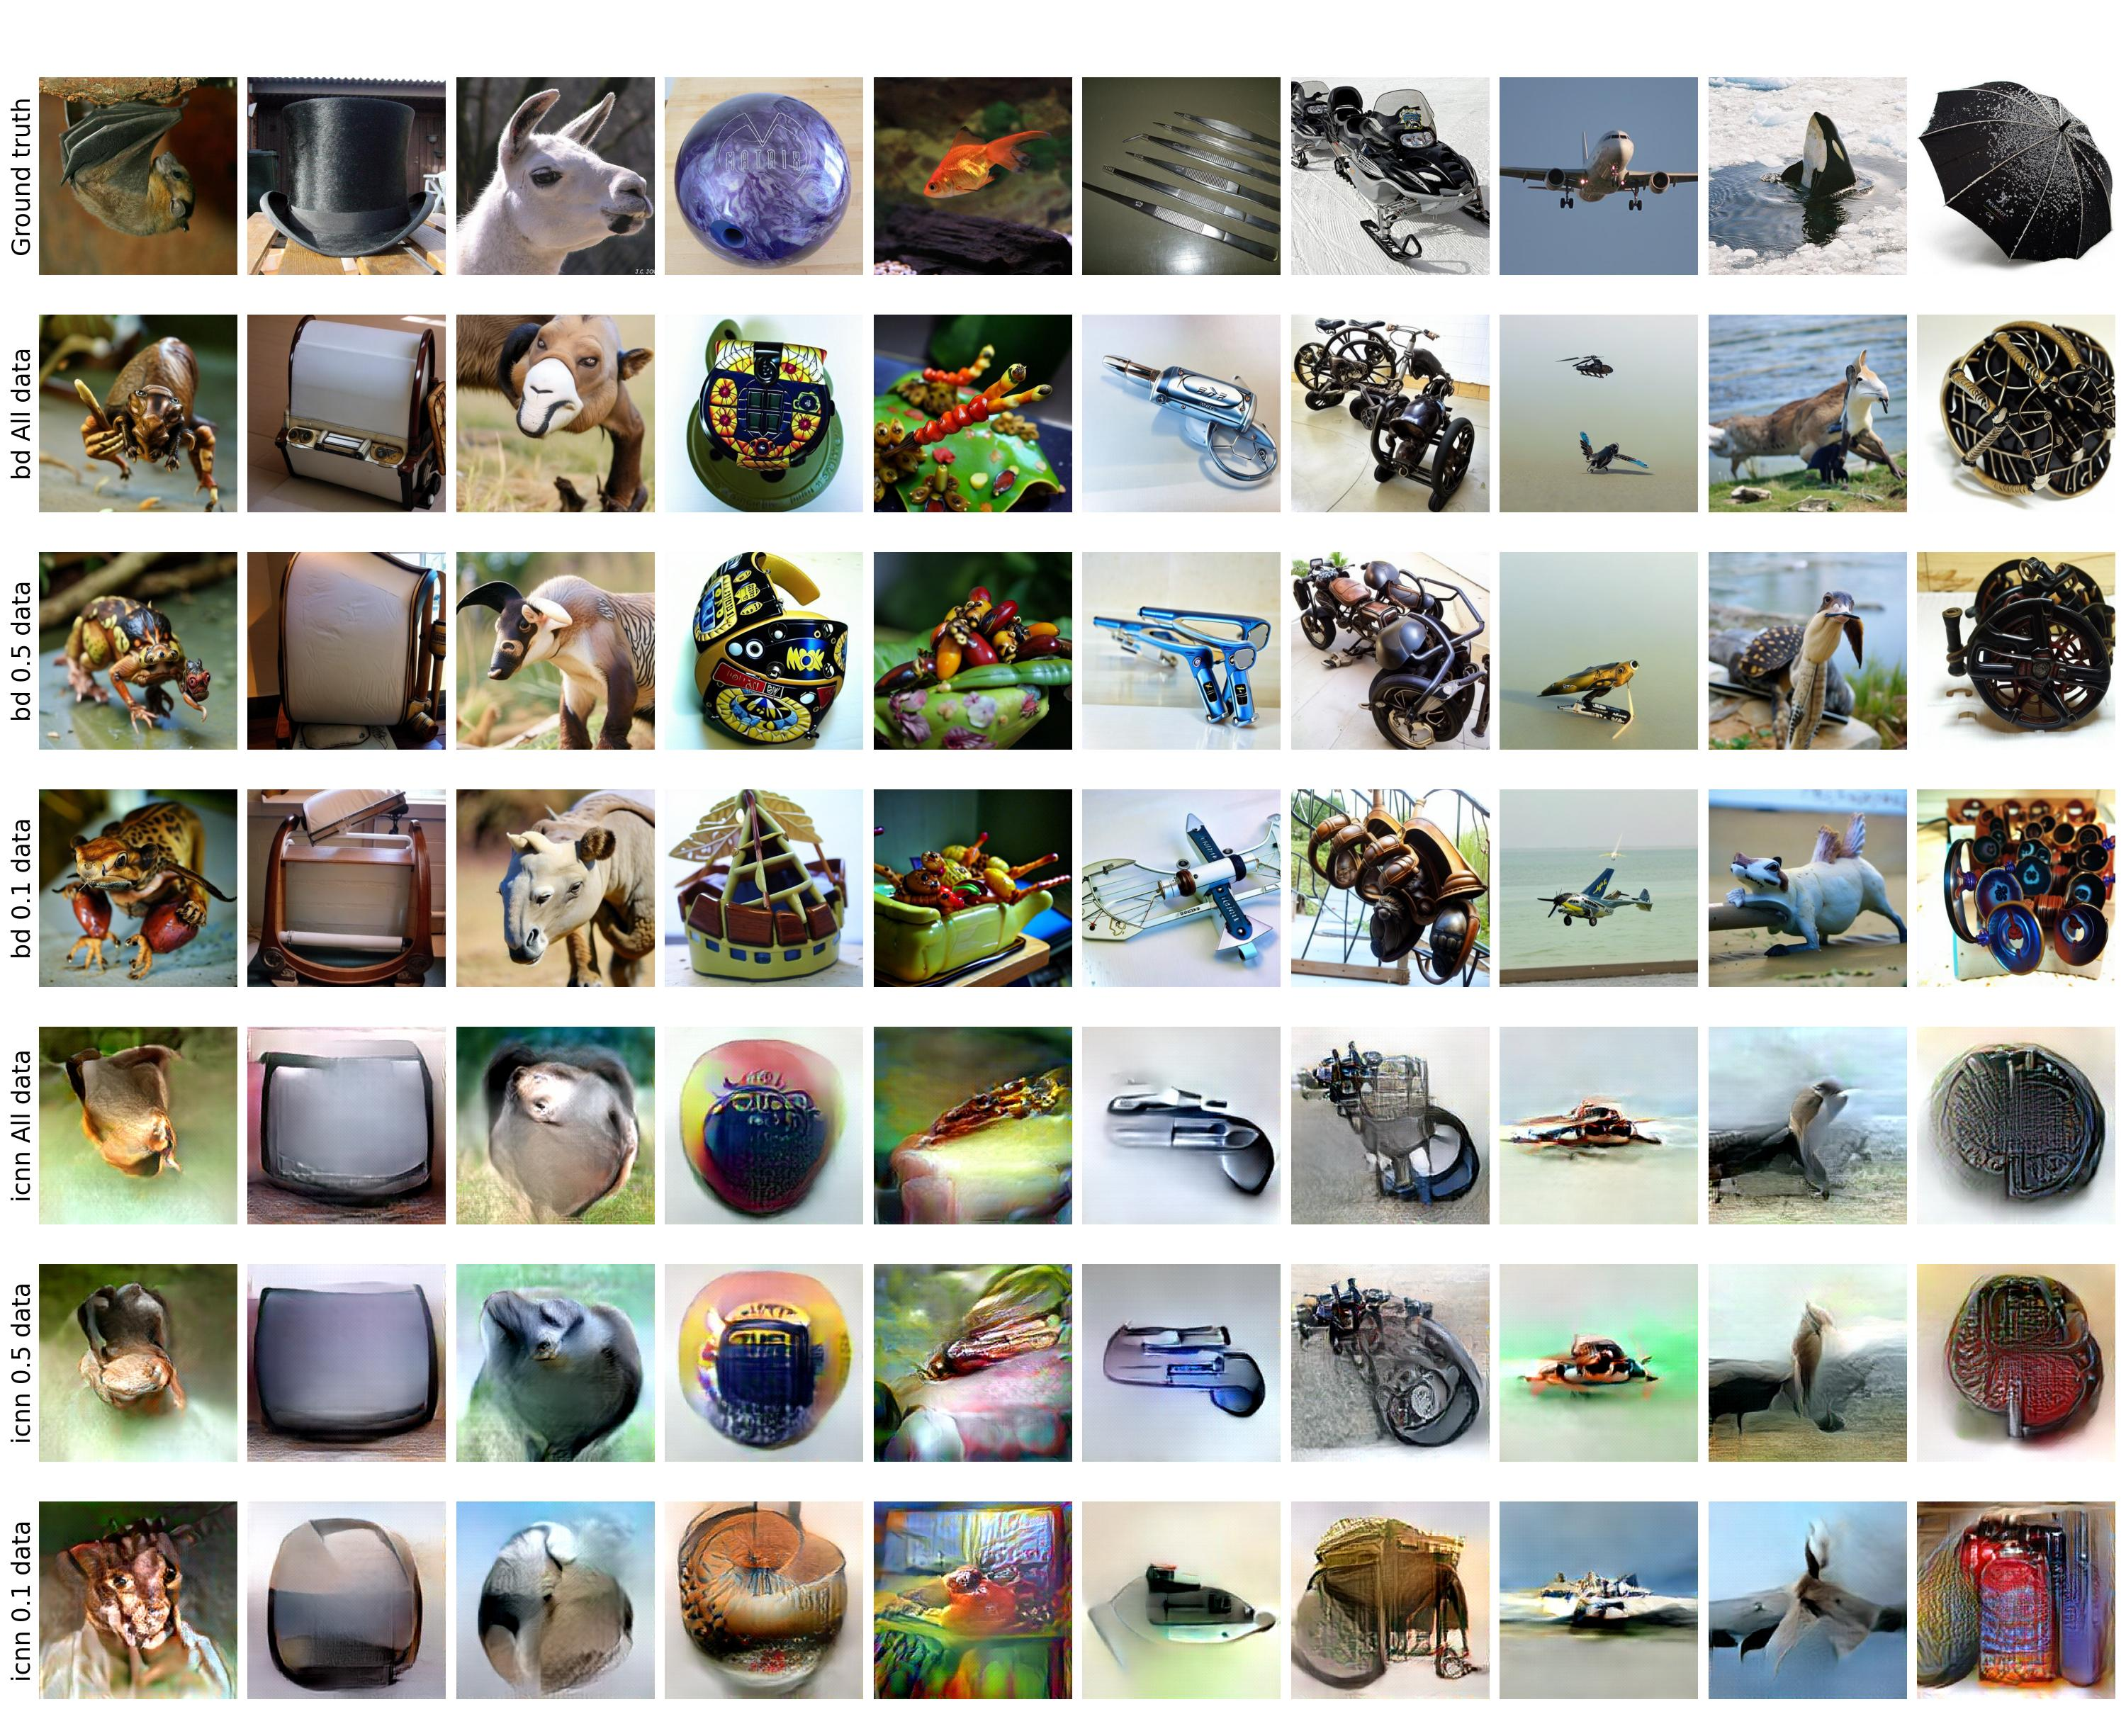
\includegraphics[width=1\textwidth]{plots/dropout_qual_random_test.JPEG}
    \caption{Qualitative results with different levels of random dropout on natural test images}\label{fig:dropout_qual_random_test}
\end{figure}

% 3.5 Reconstruction Random Qual Plot art
\begin{figure}[ht]
    \centering
    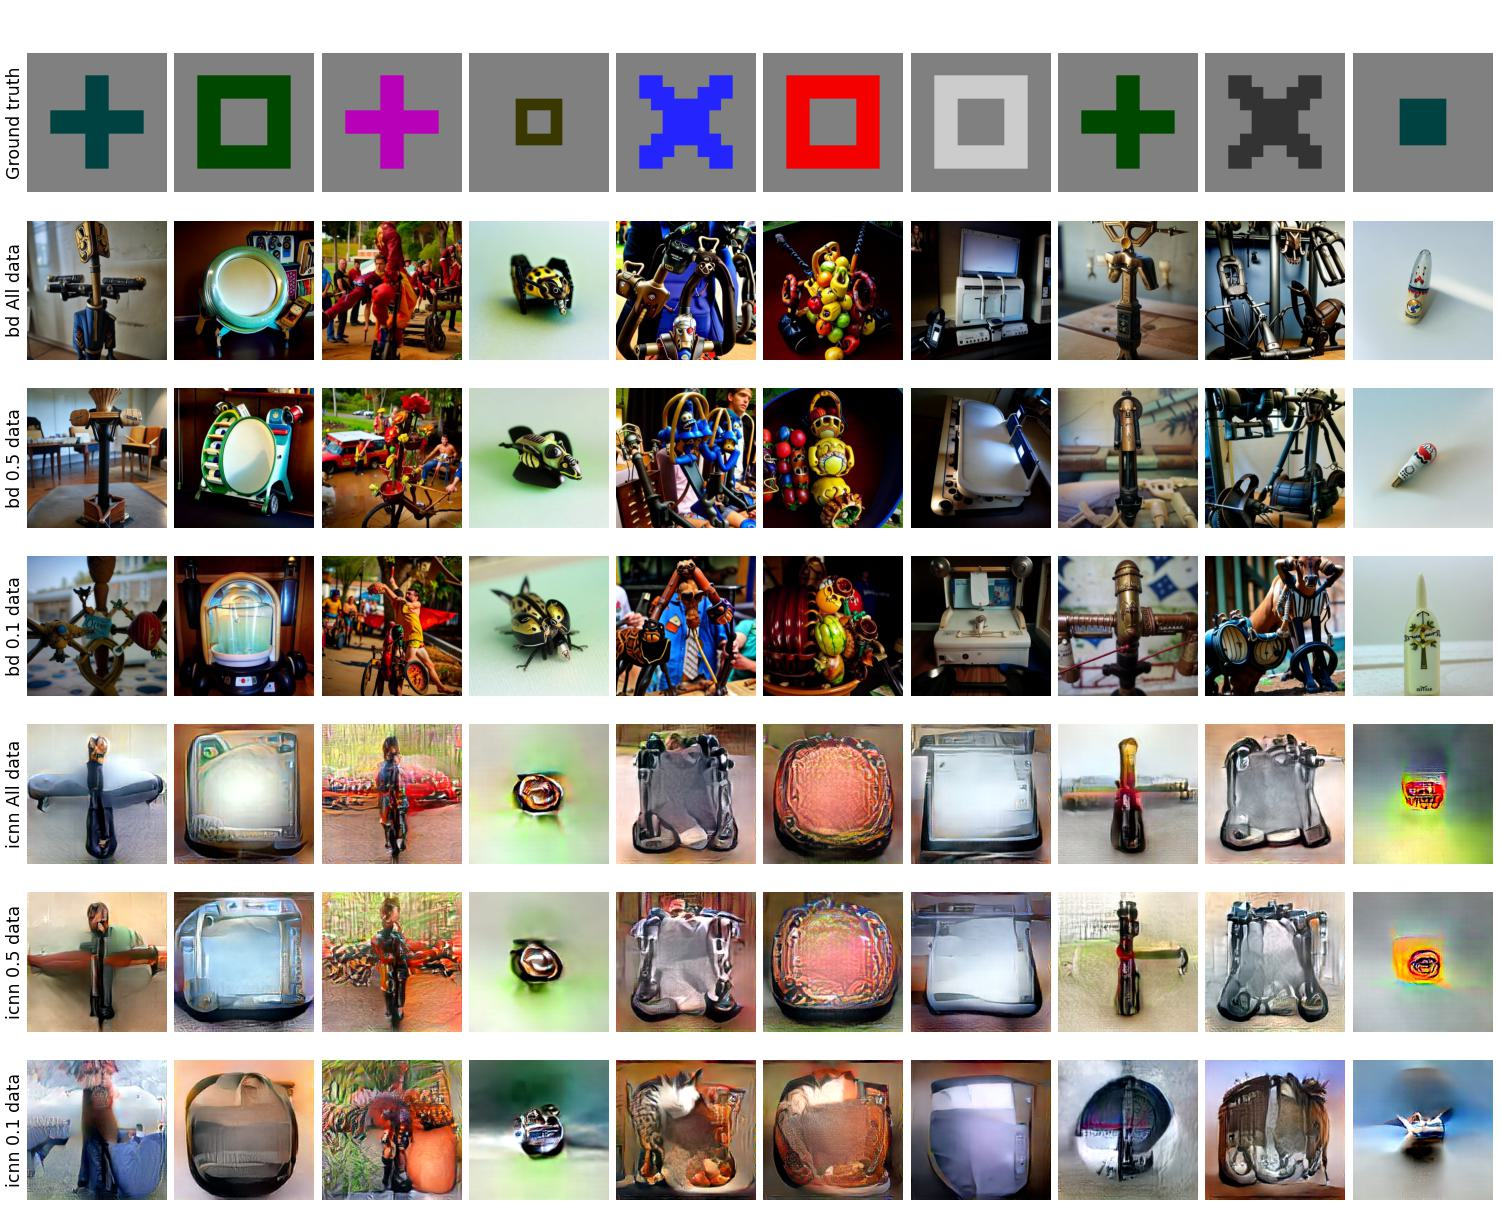
\includegraphics[width=1\textwidth]{plots/dropout_qual_random_art.JPEG}
    \caption{Qualitative results with different levels of random dropout on artificial shapes}\label{fig:dropout_qual_random_art}
\end{figure}

The qualitative performance of the reconstructions with different training set sizes can be seen in Figure~\ref{fig:dropout_qual_random_test} for the natural test images and in Figure~\ref{fig:dropout_qual_random_art} for the artificial shapes. It can be seen that even with only 10\% of the training images, distinctive features of the images can be reconstructed. However, it can also be seen that the quality of the reconstructions improves as the amount of training data increases. For example, the Brain Diffuser is not yet able to correctly classify the snowmobile as a vehicle with a small amount of training data, or the outlines of the goldfish are not yet nearly correct with the ICNN.\@ Interestingly, the reconstruction of the brain diffuser's aircraft is better with a small number of training samples than with the full data set. This is probably because the VDVAE, which produced artefacts for this image, still works with the small number of training samples. For the artificial shapes, there is a visible improvement in the quality of the reconstruction, especially for the ICNN, as the number of training samples increases. This goes along with the quantitative results.

In summary, it can be said that the performance in decoding and reconstruction can usually be significantly improved with an increasing number of training samples. In our example, many effects become visible in the step between 25\% and 50\% of the training data set, and in some cases the performance starts to saturate from this point on. For the following experiments, therefore, the data set should not contain more than 50\% of the training samples, in order to still have potential for performance improvement. At the same time, the training data set should not be smaller than 25\%, otherwise the decoding may not work well enough for testing.

\subsubsection{Diversity based Data-Subsampling}

For this work, the data should be subsampled as diversely as possible in order to produce a reduced dataset that can beat a randomly subsampled dataset in terms of decoding and reconstruction performance. In this work, a multi-step subsampling procedure is chosen: First, all training images are transformed into a latent feature space (within this feature space, an attempt is made to maximise diversity). Then, the nonlinear dimension reduction algorithm UMAP\cite{mcinnesUMAPUniformManifold2018} is used to reduce the dimensionality of the training images embedded in the feature space to two dimensions. The data in the UMAP space is then divided into $k$ clusters using k-means\cite{1056489} clustering (where $k$ is the number of images to be subsampled). For each of the $k$ clusters, the centroid of all $n$ images in that cluster is determined. Finally, for each cluster, the image with the smallest Euclidean distance to the centroid is selected. Using this procedure, $k$ images can be subsampled, where $k$ is arbitrary but must be less than the total number of training images. However, it should be clear that $k$ clusters cannot reasonably be found in the selected feature space; for example, if $k$ is selected very high (about 50\% of the dataset), only 2 images would be present in each cluster. To ensure that the subsampling algorithm can produce a meaningful subselection of the training set, k should be chosen as small as possible. Given the results of the random subselection baseline in the previous chapter, $k$ is set to 25\% (i.e. 300) of the images in the training set. 

% 4 UMAP
\begin{figure}[ht]
    \centering
    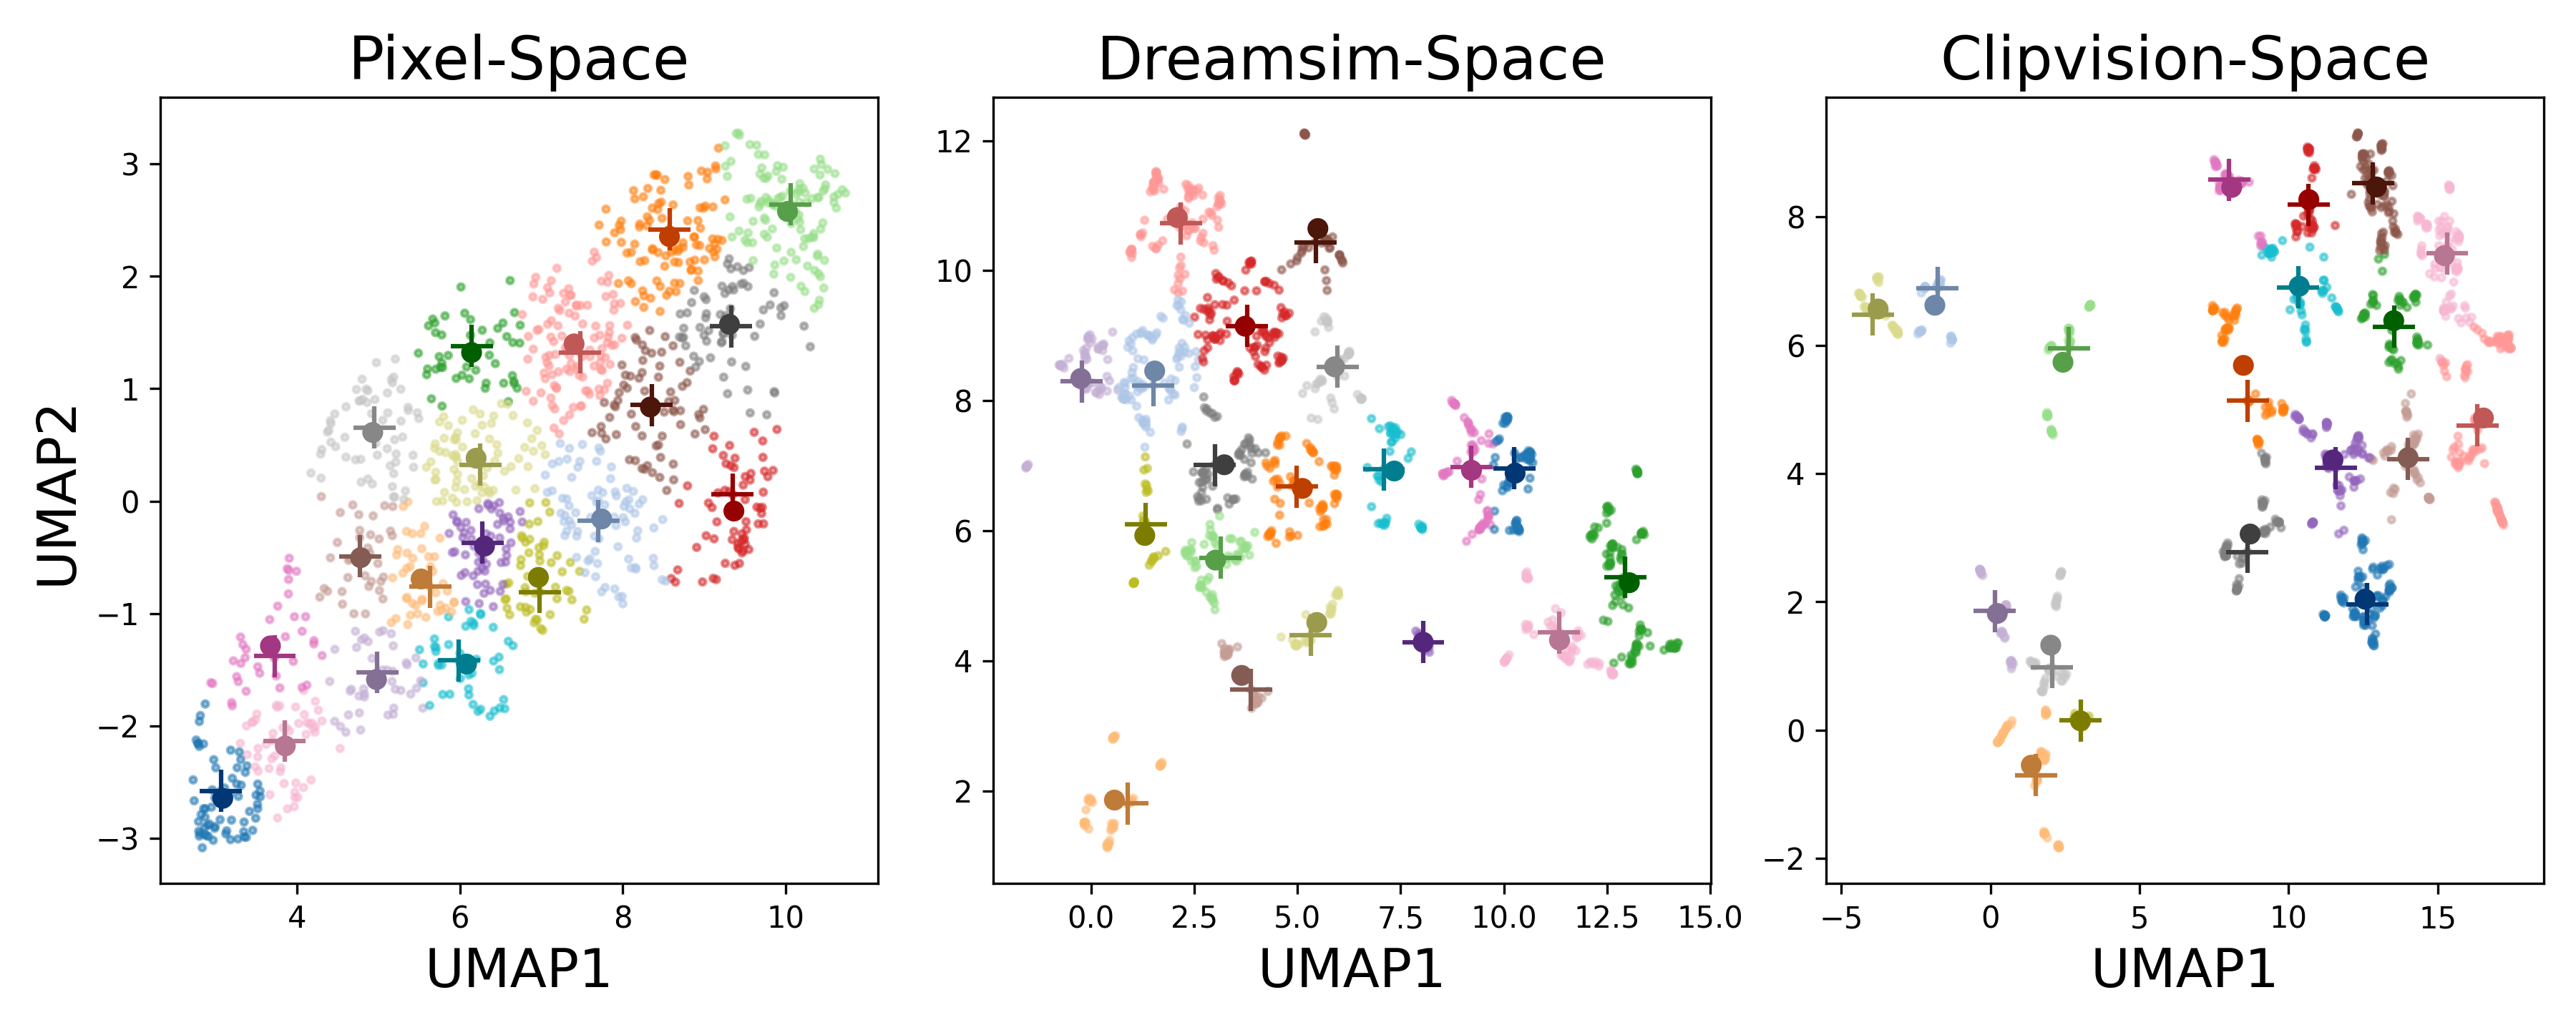
\includegraphics[width=0.9\textwidth]{plots/dropout_umap.png}
    \caption{UMAP + k-means of Pixel-Space, Dreamsim and Clipvision Space}\label{fig:dropout_umap}
\end{figure}




The feature space in which the training images are initially embedded is freely selectable. To follow the logic of the evaluation criteria, a low-level, a mid-level and a high-level representation are chosen. For the low-level representation, the images (resized to 200$\times$200 pixels) are simply concatenated into a one-dimensional vector, so that the subsequent UMAP algorithm can only reduce the dimensions at the pixel level (this procedure was successfully applied by the authors of UMAP to the MNIST dataset). For the mid-level representation, the training images are embedded with Dreamsim\cite{fuDreamSimLearningNew2023}, for the high-level representation, the training images are embedded in clip-space using clipvision\cite{radfordLearningTransferableVisual2021}. Thus, all images are transformed into one-dimensional vectors whose dimensionality is reduced using UMAP and clustered using k-means. 
The results of the selection process are shown as an example in Figure~\ref{fig:dropout_umap}. In the plots, the number of clusters has been set to $k=20$ for visualisation purposes. Each point in the plot represents a slice of the training data set in UMAP space. The clusters are coloured differently. The centroid of each cluster is shown as a circle and the image closest to the centroid is marked with a cross. In Dreamsim and Clipvision space, the different clusters are already clearly separated from each other in the two dimensions of UMAP, while the result in pixel space has divided the images comparatively homogeneously, which may indicate that the UMAP dimension reduction has not worked optimally (this can probably be explained by the high number of dimensions in pixel space 200$\times$200$\times$3 colour channels = 120000). 
Subsamples with 25\% (300 images) of the training data set were extracted for each of the feature spaces using the method described above. Figure~\ref{fig:dropout_similarity_plot} shows the most similar image in the reduced dataset for each feature space for ten images from the input dataset (left column). This shows the differences in sampling in the three feature spaces: in the Dreamsim and Clipvision spaces, the images are relatively similar to the original. However, the differences between the mid-level and high-level similarities become clear. For example, in the case of the revolver in the first image, Dreamsim selects a gun that is relatively similar in the image, but is the wrong type. Clipvision selects an image that is a better semantic match because it also shows a revolver, even though the remaining visual similarity is lower (colour of the gun, partially covered by a hand). This difference between clipvsion and Dreamsim can also be seen in other images. In pixel space, however, the subjective similarity between the original and the sample is lower. In the third image, for example, the original shows an ear with white headphones, while the most similar image in pixel space is a goose with a long white neck. The low-level match between the images is presumably an elongated white object in the middle. 

% 5 Umap Subselection Similarity from low_level_clustering.py
\begin{figure}[ht]
  \centering
  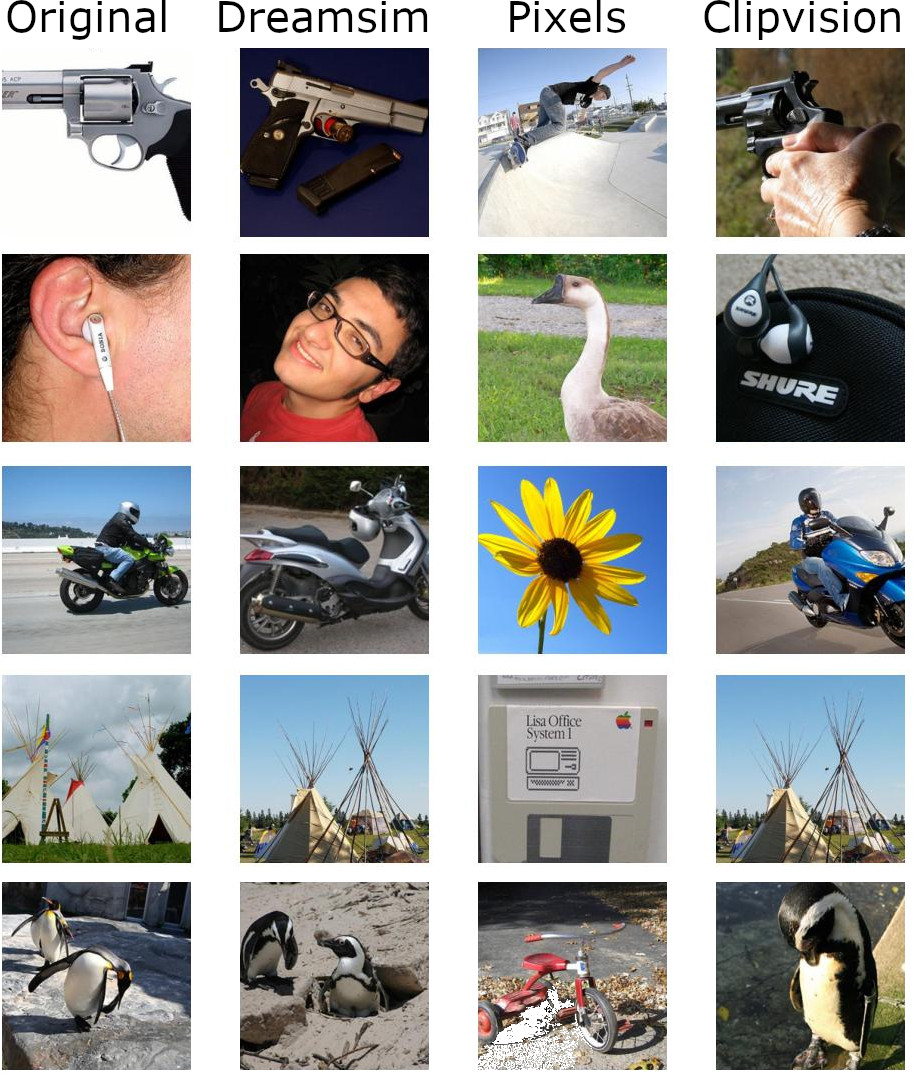
\includegraphics[width=0.6\textwidth]{plots/dropout_similarity_plot.JPEG}
  \caption{Most similar image to original in multiple subspaces}\label{fig:dropout_similarity_plot}
\end{figure}

In order to ensure that the subselection has indeed increased the diversity in the feature space, it is validated quantitatively. For this purpose, a new metric is defined, the average minimum distance to all training samples (avg\_min\_dist). It is defined as follows

\[
\text{avg\_min\_dist}
= \frac{1}{n_{\text{all}}}
  \sum_{i=1}^{n_{\text{all}}}
    \min_{1 \le j \le n_{\text{sub}}}
      \Bigl\lVert f(\mathbf{x}_i) - f(\mathbf{y}_j) \Bigr\rVert
\]

\[
\begin{aligned}
n_{\text{all}} &:=
  \text{number of images in the full set}, \\
n_{\text{sub}} &:=
  \text{number of images in the subsample}, \\
\mathbf{x}_i &:=
  \text{the $i$-th image in the full training dataset}, \\
\mathbf{y}_j &:=
  \text{the $j$-th image in the subsample}, \\
f &:=
  \text{embedding function from image feature space (Pixels, clipvision, dreamsim)}, \\
\|\cdot\| &:=
  \text{the Euclidean (L2) norm}.
\end{aligned}
\]

The avg\_min\_dist measures how close on average each image in the full training dataset  (embedded in the respective feature space) is to the next possible image in the subsample. If the subsample adequately represents the feature space, then for each input image there would be a comparatively close candidate in the subsample. The avg\_min\_dist was computed for all three feature spaces and is shown in Figure~\ref{fig:dropout_avg_min_distance}. For each subspace, 30 different samples were taken and the avg\_min\_dist was calculated for each sample. The figure shows that in each feature space, the subsample created using the corresponding feature space has the lowest avg\_min\_dist. The result is most ambiguous for the avg\_min\_dist in the pixel feature space, but again the subsample created using the pixel space has the lowest avg\_min\_dist. The avg\_min\_dist for dreamsim and clipvision are always comparatively close, which makes sense since dreamsim is partly based on clipvision\cite{fuDreamSimLearningNew2023}. 

\begin{figure}[ht]
    \centering
    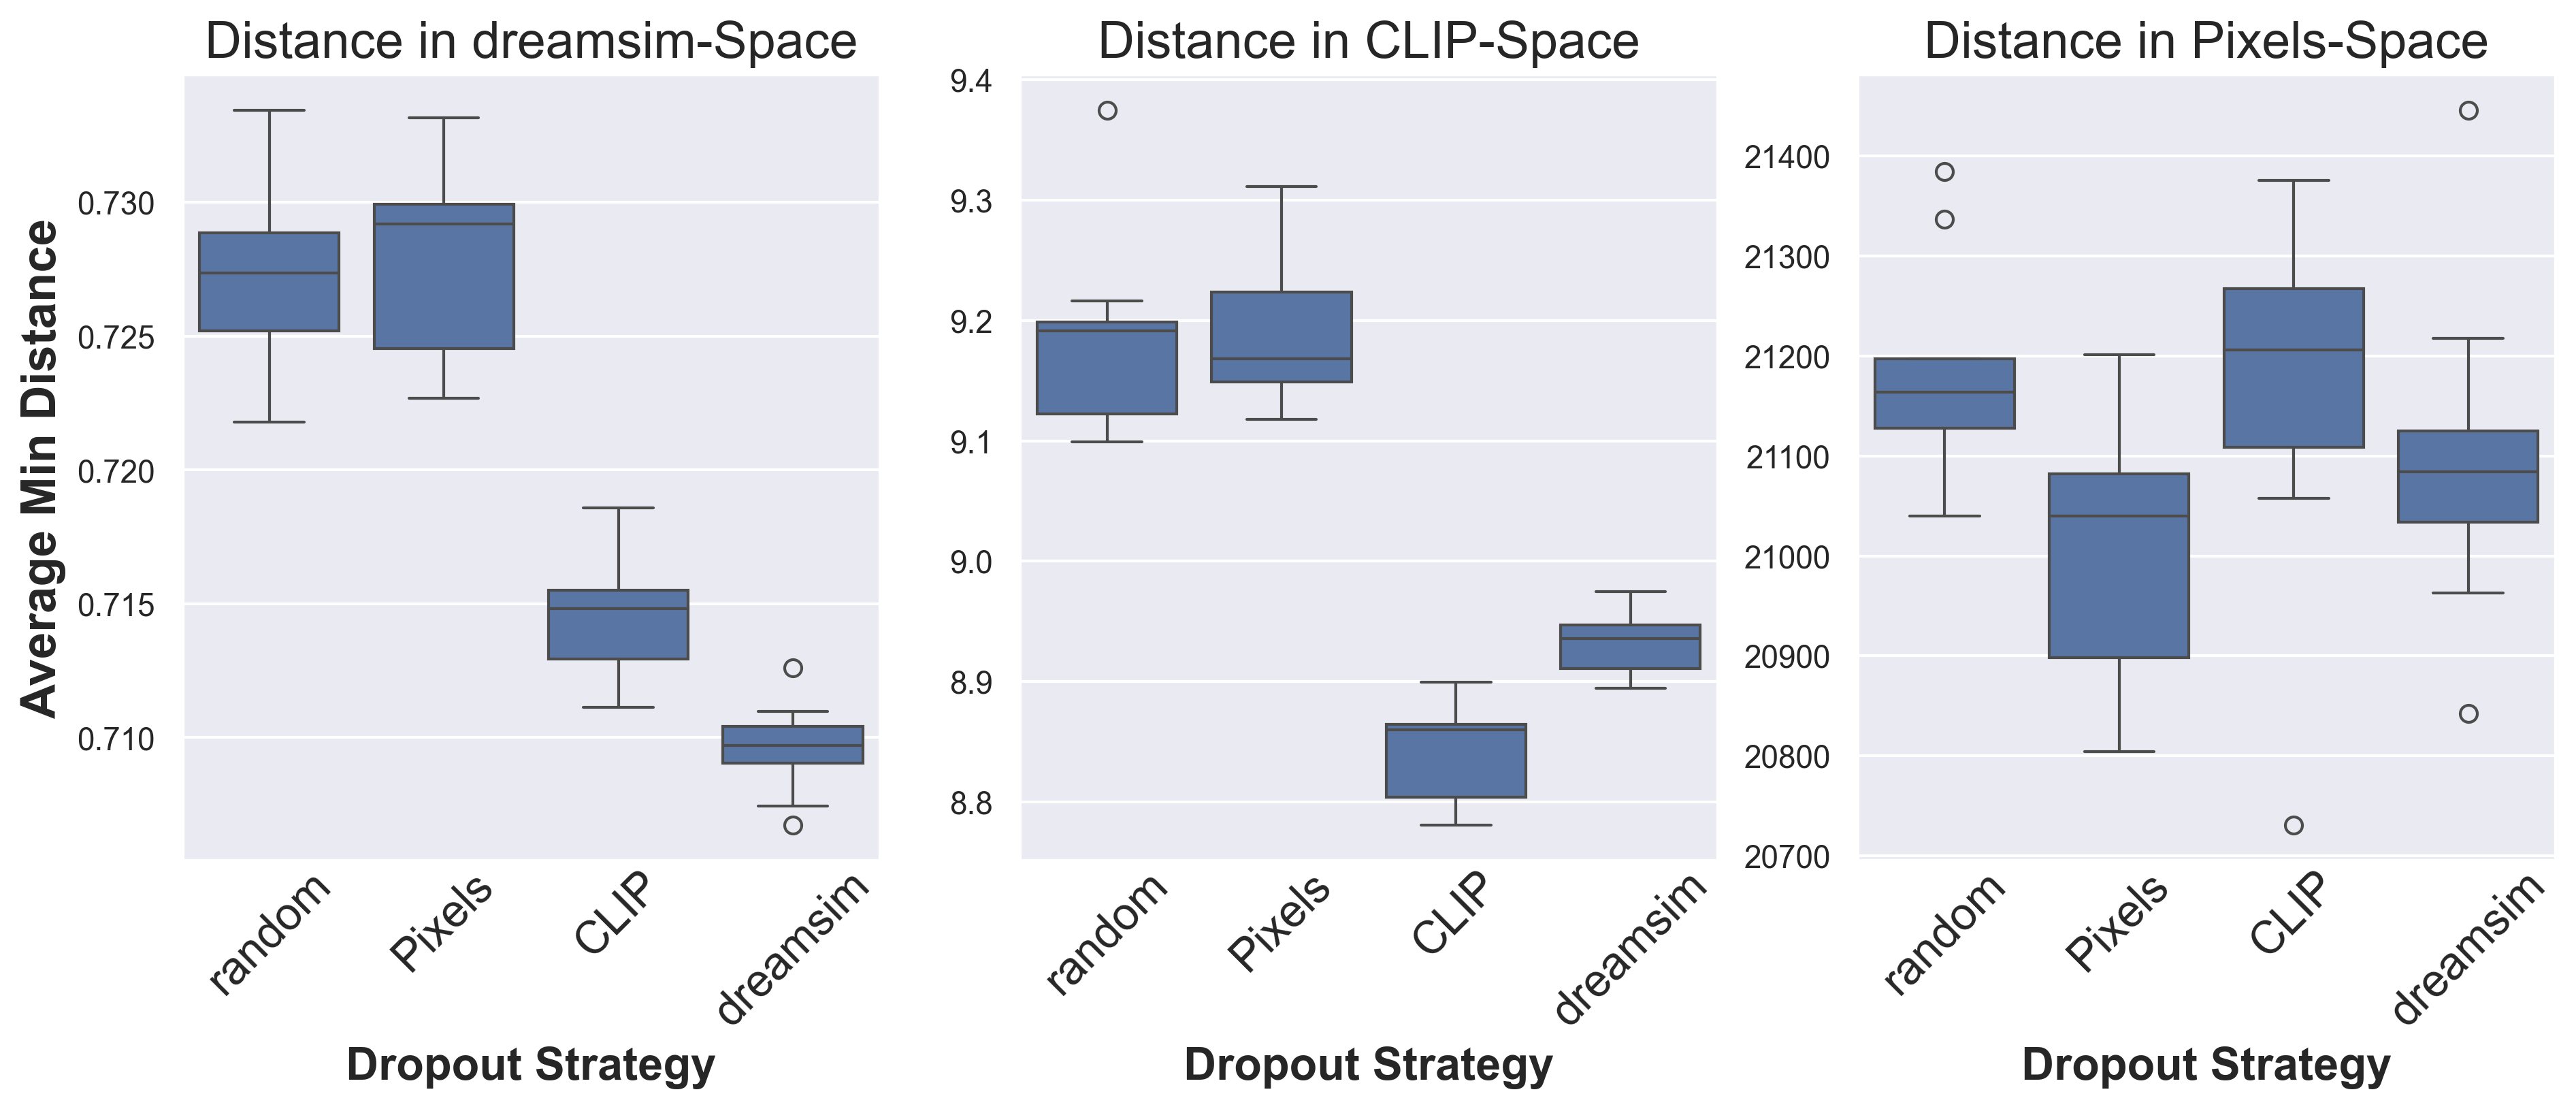
\includegraphics[width=1\textwidth]{plots/dropout_avg_min_distance.png}
    \caption{Avg-min-distance of subsample to All Training Images}\label{fig:dropout_avg_min_distance}
\end{figure}


In summary, the qualitative and quantitative review showed that the diversity-based subsampling method is successful in increasing the diversity in the respective subspace. For each feature space, the subsample with the lowest avg\_min\_dist in the validation (i.e.\ best representing the entire feature space) is used for further analysis.


\subsection{Results}
The three generated subspaces were used below to train the translator and reconstruct images for each of the five subjects. To provide an adequate baseline, the results of the three subspaces are each compared with a random subselection. 

\subsubsection{Decoding results}
The performance of the three trained translators of the brain diffuser and the VGG19 features of the ICNN algorithm is shown in Figure~\ref{fig:dropout_eval_translator_test} for the natural test images and in Figure~\ref{fig:dropout_eval_translator_art} for the artificial shapes. The results are shown for all four different dropout strategies (random subsample and samples based on the three feature spaces). For the natural test images, the performance of all subsamples is above the random probability of 0.5. However, for the three translators of the brain diffuser, there are no discernible differences in performance between the different dropout strategies. Only the ICNN translator shows that performance can be slightly improved with a targeted diversity-based subsampling strategy. However, in this case too, there is no significant difference between the three feature spaces.

% Now the Eval Results
% 7.1 Eval Translator test
\begin{figure}[ht]
  \centering
  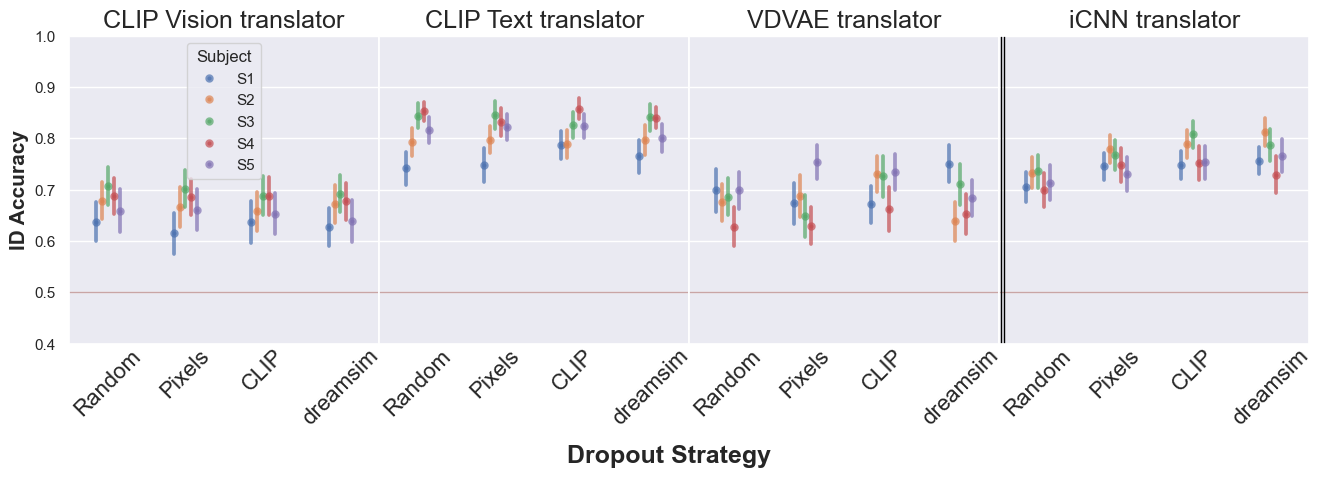
\includegraphics[width=1\textwidth]{plots/dropout_eval_translator_test.png}
  \caption{Translator performance (0.25 data fraction) for Natural Test Images}\label{fig:dropout_eval_translator_test}
\end{figure}

The artificial shapes in Figure~\ref{fig:dropout_eval_translator_art} show that the two clip translators are not able to predict the features significantly beyond random probability. This is independent of the subsampling space. The performance of the VDVAE translator is slightly better, with all subsamples tending to be better than the random probability. In particular, the performance of the low-level pixel feature space seems to have a slight advantage over the other subsampling strategies. For the ICNN translator, on the other hand, the effect of the natural test images seems to have been reversed; for the Pixel and Dreamsim feature spaces, the performance even looks slightly worse than with random subsampling. Within the clipvision feature space, the variance between the subjects is really high, thus the results cannot easily be interpreted.

\begin{figure}[ht]
  \centering
  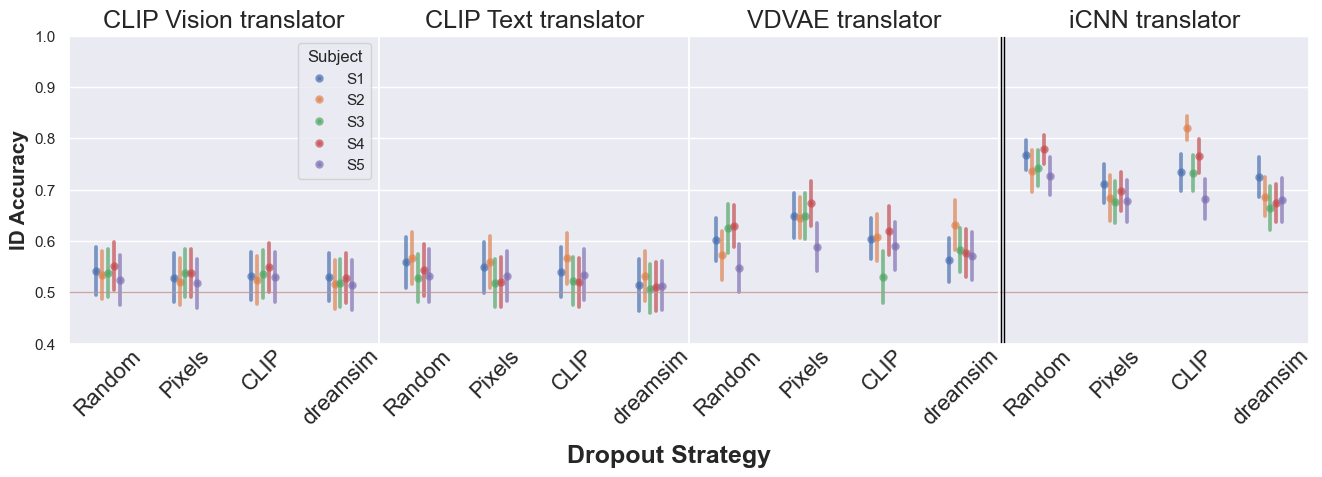
\includegraphics[width=1\textwidth]{plots/dropout_eval_translator_art.png}
  \caption{Translator performance (0.25 data fraction) for Artificial Shapes}\label{fig:dropout_eval_translator_art}
\end{figure}


\subsubsection{Reconstruction Results}

\begin{figure}[ht]
  \centering
  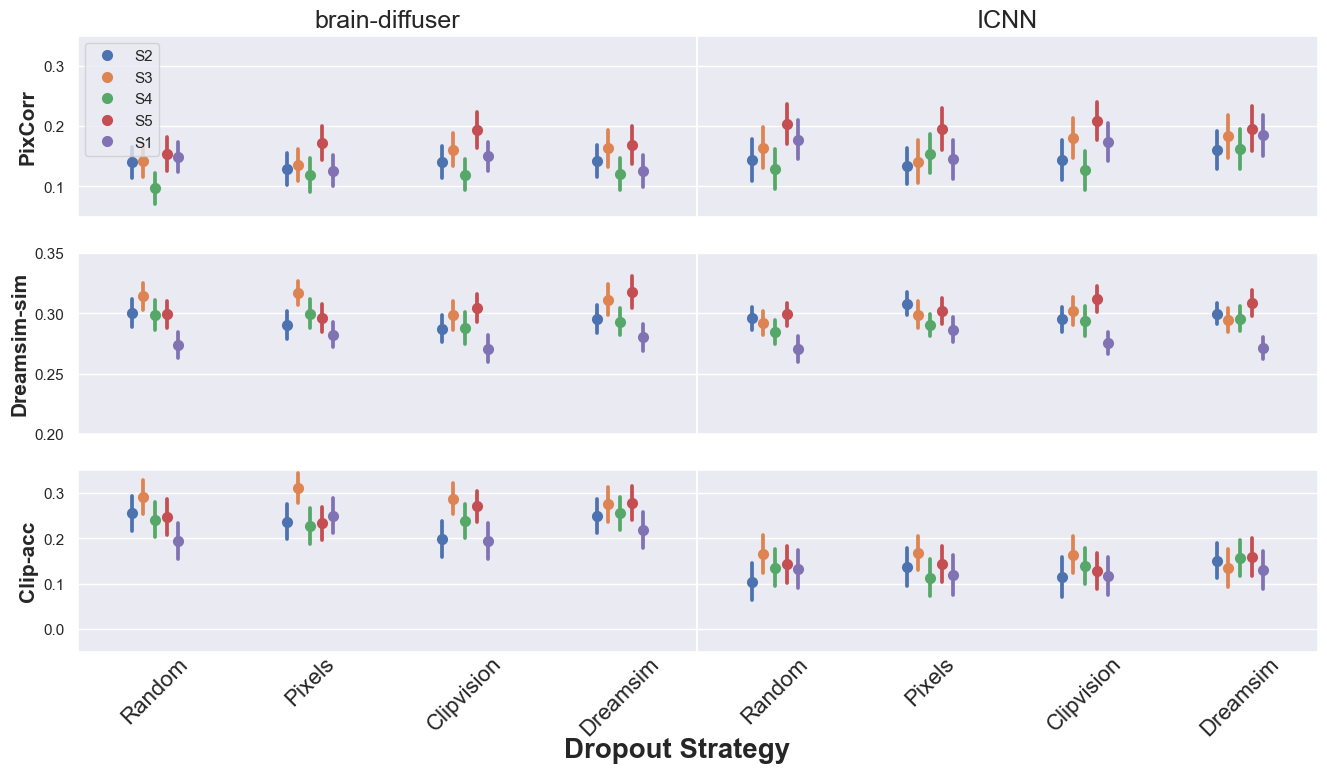
\includegraphics[width=1\textwidth]{plots/dropout_eval_reconstruction_test.png}
  \caption{Reconstruction Performance (0.25 data fraction) for Natural Test Images}\label{fig:dropout_eval_reconstruction_test}
\end{figure}

The quantitative results of the reconstructions using the four different subsamples are shown in Figure~\ref{fig:dropout_eval_reconstruction_test} for the natural test images and in Figure~\ref{fig:dropout_eval_reconstruction_art} for the artificial shapes. The three previously described criteria of PixelCorrelation, Dreamsim-similarity and Clip-Accuracy are specified for the Brain Diffuser and ICNN algorithms respectively. For the natural test images, there is no discernible difference between the random subselection and the three diversity-based subsamples for the Brain Diffuser in any of the three metrics. The results are similar for the ICNN.\@ Although the translator performance was improved beforehand, these effects seem to have only a minor impact on the reconstruction performance. Only with the help of the Dreamsim-sim metric is there a slight increase in performance across all three feature spaces in contrast to the baseline. There are again no differences between the feature spaces however.

\begin{figure}[ht]
  \centering
  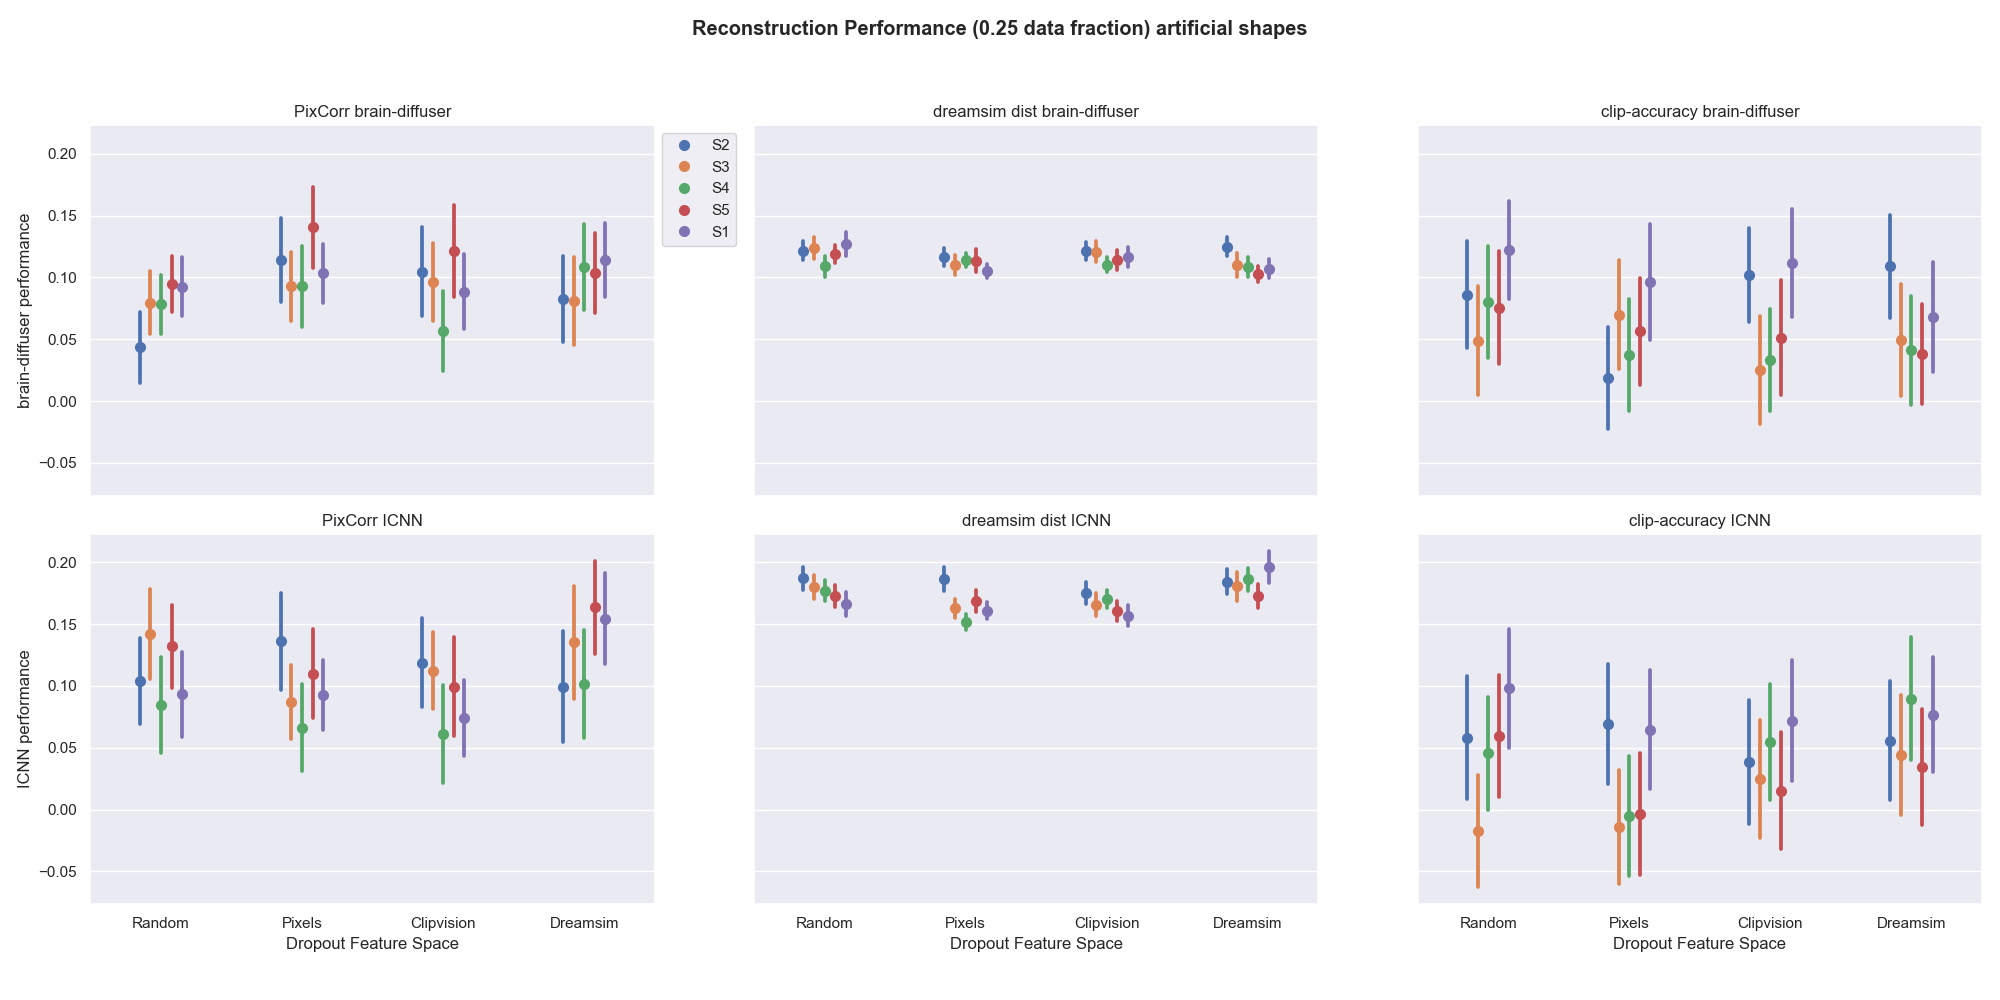
\includegraphics[width=1\textwidth]{plots/dropout_eval_reconstruction_art.png}
  \caption{Reconstruction Performance (0.25 data fraction) for Artificial Shapes}\label{fig:dropout_eval_reconstruction_art}
\end{figure}


Also for the artificial shapes in Figure~\ref{fig:dropout_eval_reconstruction_art}, the differences in reconstruction performance between the different feature spaces are small. For the brain diffuser it looks as if the pixel correlation with a dropout is slightly increased in the pixel subspace compared to the baseline. There are no visible differences in the other metrics. In the ICNN, the Dreamsim similarity appears slightly reduced in Pixels subspace and Clipvision subspace compared to the baseline. There are no visible differences in the Dreamsim subspace. 

\begin{figure}[ht]
  \centering
  \includegraphics[width=1\textwidth]{plots/dropout_qual_eval_icnn_test.JPEG}
  \caption{Qualitative Results for different dropout strategies with the ICNN on natural test images}\label{fig:dropout_qual_eval_icnn_test}
\end{figure}

As the quantitative results of the reconstruction performance suggest, a qualitative assessment of the differences in the reconstruction is difficult. The ICNN results for the natural test images are shown in Figure~\ref{fig:dropout_qual_eval_icnn_test} and for the artificial shapes in Figure~\ref{fig:dropout_qual_eval_icnn_art}. Differences in the quality of the reconstruction are difficult to determine; although it is clear that at least some reconstruction quality can be achieved in all conditions, the slight improvement of the feature spaces in contrast to the random baseline  seen in the quantitative results is not immediately apparent in the actual images. Likewise, for the artificial shapes in Figure~\ref{fig:dropout_qual_eval_icnn_art}, the slight degradation in the feature space results compared to the random sample is not directly apparent from the qualitative results. The quantitative results for the brain diffuser were even more ambiguous, so no major differences can be seen in the qualitative analysis of the images. The reconstructed images for the brain diffuser can be found in the appendix (Figure~\ref{fig:dropout_qual_eval_bd_test} for the natural test images and Figure~\ref{fig:dropout_qual_eval_bd_art} for the artificial shapes).


\begin{figure}[ht]
  \centering
  \includegraphics[width=1\textwidth]{plots/dropout_qual_eval_icnn_art.JPEG}
  \caption{Qualitative Results for different dropout strategies with the ICNN on artificial shapes}\label{fig:dropout_qual_eval_icnn_art}
\end{figure}

\subsection{Discussion}

% Results Zusammenfassung:

% brain-diffuser:
%   - Bei den brain-diffuser decodern hat sich kein großer Unterschied gezeigt zwischen den subsamples
%     - Low level Pixel Space hat decoding beim low level VDVAE mutmaßlich etwas gesteigert bei den artificial Shapes. Der Effekt scheint aber nicht unbedingt stabil zu sein und könnte zufällig sein.
%   - Bei der Reconstruction
%     - Natural Test Images kein Effekt
%     - Artificial Images in der pixCorr leicht verbesser

% icnn:
%   - Beim ICNN kann der Decoder verbessert werden durch das subsampling beim Test Datensatz
%     - Kein Unterschied zwischen den Subsampling methoden aber
%     - Bei ICNN ist der Zusammehang bei den artificial Shapes sogar umgedreht (also schlechter beim Subsampling)
%   - Reconstruction ist bei natural test images verbessert
%     - bei Artificial Shapes tendenziell verschlechtert
  
The hypotheses could mostly not be confirmed, but some interesting phenomena occurred. For the brain diffuser, there were generally few differences between the different subsamples. Only for the artificial shapes could the decoder for the translator and also the pixel correlation of the reconstruction be increased by low-level subsampling. This is consistent with the hypothesis that low-level subsampling improves low-level reconstruction. However, as this effect can only be measured with the pixel correlation, it should be treated with caution and could only have occurred by chance. With the ICNN, however, the results were somewhat clearer. In the case of the natural test images, the decoder could be improved by any type of subsampling, and the subsequent reconstructions could also be improved (measured with Dreamsim). Interestingly, this effect is exactly the opposite for the artificial shapes. Here, diversity-based subsampling even seems to be disadvantageous compared to random subsampling: both the decoder and the reconstruction performance decrease compared to the baseline. 

\subsubsection{Exploring the influence of monotone training data}
In the following, we will further investigate why the performance of the artificial shapes is presumably reduced by diversity-based subsampling. A closer look at the training images reveals that there are some images that show individual central objects with a monotonous (usually white) background. It could be that these are similar in concept to the artificial shapes. In this sense, the artificial shapes would not really be out-of-distribution samples, because a monotone background of the training images is not really natural either. It is investigated whether these images have a significant influence on the reconstruction. In order to test this, a new, reduced training data set is created, which mainly contains these images. A simple algorithm is used to identify these images in the training dataset automatically: The colour values for each pixel in all images are counted, and then the images are sorted according to how often the most frequent pixel occurs in each image (so an image with a white background would have the colour white, which occurs extremely often). In figure~\ref{fig:dropout_discussion_monohetero_qual}, the 5 most monotonous images found by the algorithm (i.e.\ those where the most frequent colour occurs very often) are compared with the 5 most heterogeneous images (i.e.\ those where the colours are more evenly distributed). As can be seen, the subdivision of the images using this algorithm worked well. In the following, decoders consisting of 0.25 (i.e. 300 images) of the training data for the most homogeneous and heterogeneous as defined by the algorithm explained above set are trained again.


\begin{figure}[ht]
  \centering
  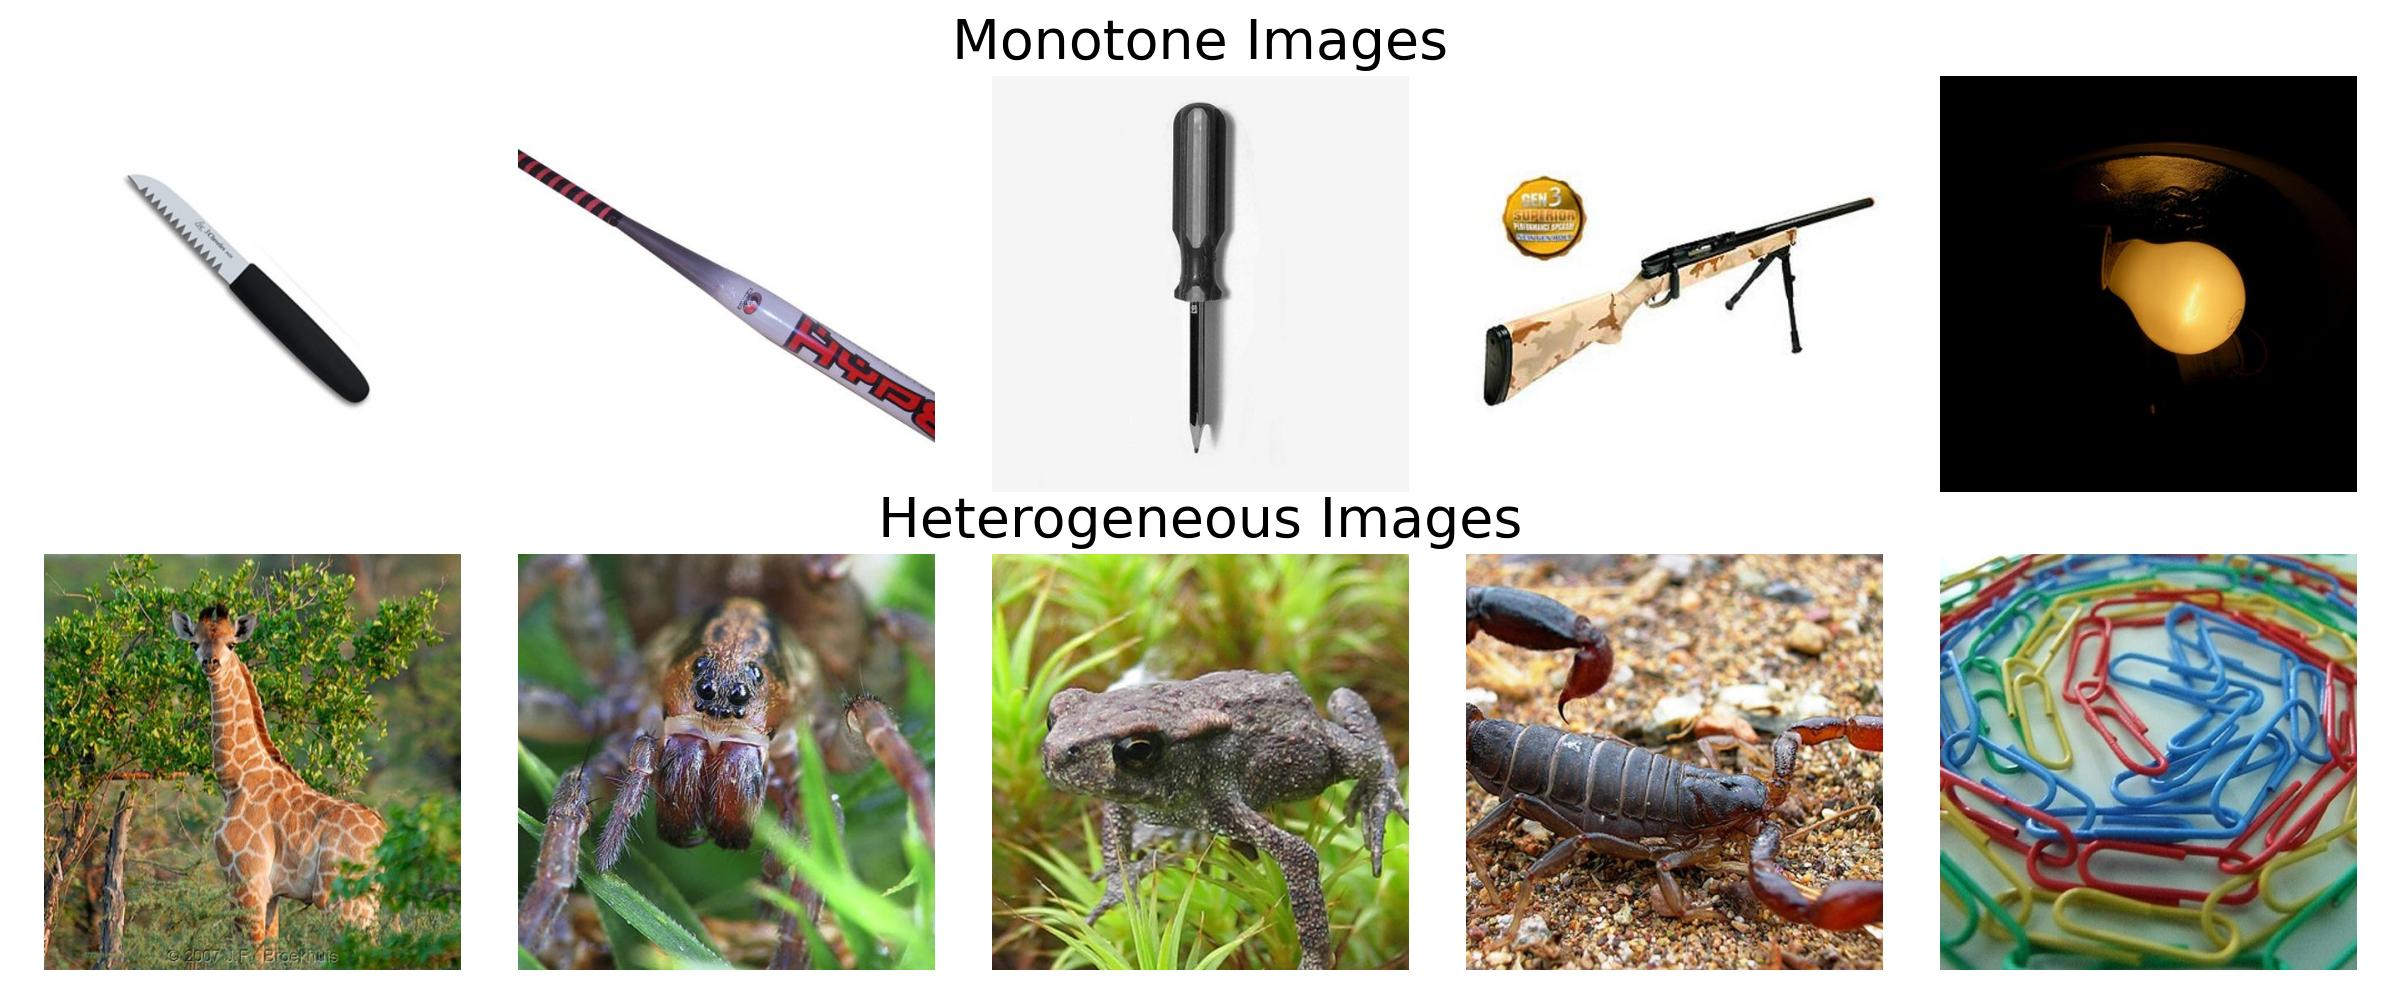
\includegraphics[width=1\textwidth]{plots/dropout_discussion_monohetero_qual.jpeg}
  \caption{Comparison of monotone and heterogeneous training images}\label{fig:dropout_discussion_monohetero_qual}
\end{figure}

\begin{figure}[ht]
  \centering
  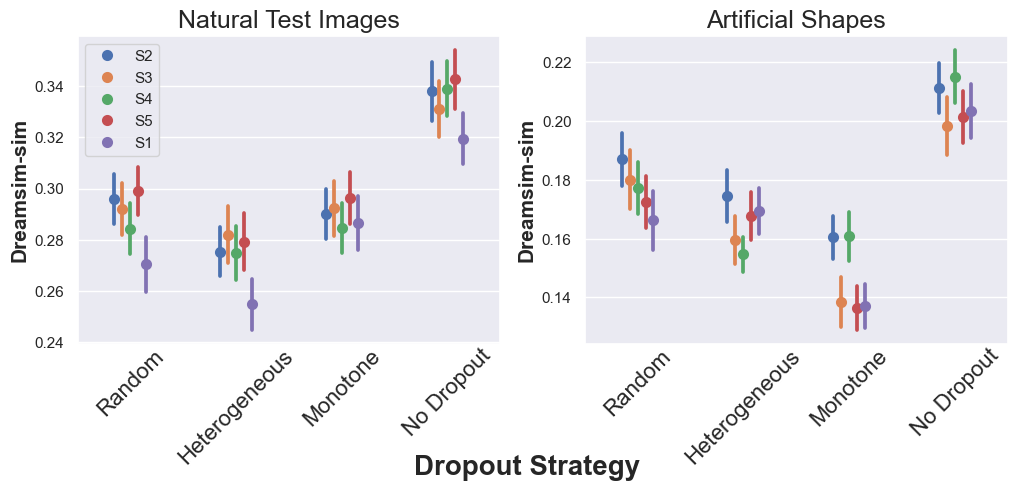
\includegraphics[width=1\textwidth]{plots/dropout_discussion_reconstruction_icnn.png}
  \caption{ICNN Reconstruction Results for monotone vs.\ heterogeneous training images}\label{fig:dropout_discussion_reconstruction_icnn}
\end{figure}


The quantitative results of the reconstructions with the monotonous and heterogeneous subsample training datasets are shown in Figure~\ref{fig:dropout_discussion_reconstruction_icnn} for the ICNN and in Figure Figure~\ref{fig:dropout_discussion_reconstruction_bd} for the brain-diffuser (the results for each individual decoder for the monotonous vs.\ heterogeneous data sets are shown in the appendix in figures~\ref{fig:dropout_discussion_translator_id_acc_cliptext},~\ref{fig:dropout_discussion_translator_id_acc_clipvision},~\ref{fig:dropout_discussion_translator_id_acc_vdvae},~\ref{fig:dropout_discussion_translator_id_acc_icnn}). In the case of the ICNN, random dropout performs better than both monotonous and heterogeneous subsampling. Contrary to expectation, monotonous subsampling actually performs worse than heterogeneous subsampling with artificial shapes. However, the results for the brain diffuser are quite different. As expected, random subsampling performs best for natural test images. For the artificial shapes, however, there is a clear effect: monotonous subsampling leads to significantly better performance than heterogeneous subsampling. This effect is also best illustrated by the qualitative reconstructions for the natural test images in Figure~\ref{fig:dropout_discussion_test} (the qualitative results for the artificial shapes are shown in Figure~\ref{fig:dropout_discussion_art} in the appendix): for each image reconstructed with the brain diffuser, a monochrome background can be seen in the monotonous condition. In contrast, all backgrounds show multiple details when the heterogeneous training data is used. This also shows why the results of the ICNN for the artificial shapes are not necessarily improved by using monotonous training: the reconstructions with the ICNN have a comparatively neutral background when both monotonous and heterogeneous training data are used. The insights that can be gained from this additional investigation are twofold. On the one hand, the brain diffuser can be strongly conditioned to reconstruct single objects with monotonous backgrounds, so that the performance for the artificial images can be greatly improved by the background of the images alone. On the other hand, it can be seen that the ICNN generally seems to produce images with neutral backgrounds and a central object in the middle (this can also be checked with the other qualitative results in this experiment). It therefore seems that the ICNN has a bias towards this type of image, where single central objects are displayed on a neutral background, regardless of the nature of the training data. 

\begin{figure}[ht]
  \centering
  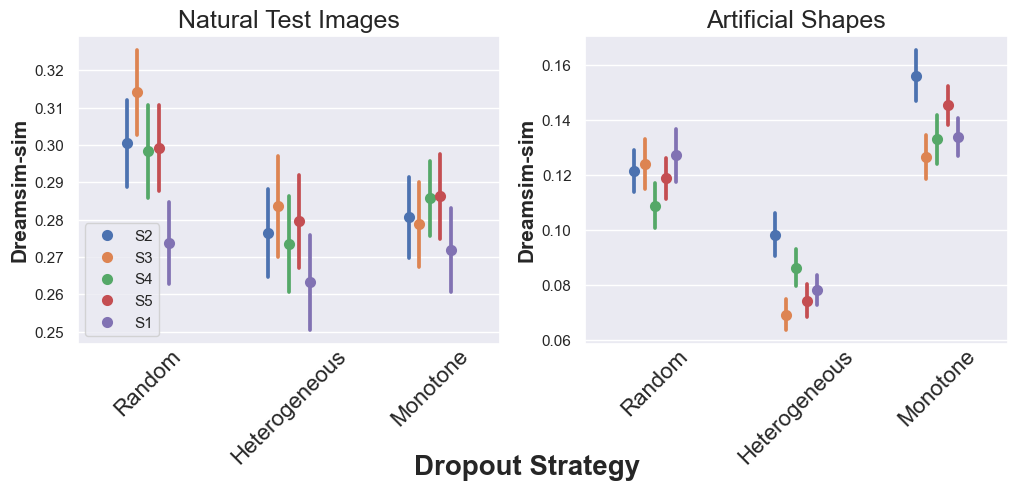
\includegraphics[width=1\textwidth]{plots/dropout_discussion_reconstruction_bd.png}
  \caption{Brain-Diffuser Reconstruction Results for monotone vs.\ heterogeneous training images}\label{fig:dropout_discussion_reconstruction_bd}
\end{figure}

\begin{figure}[ht]
  \centering
  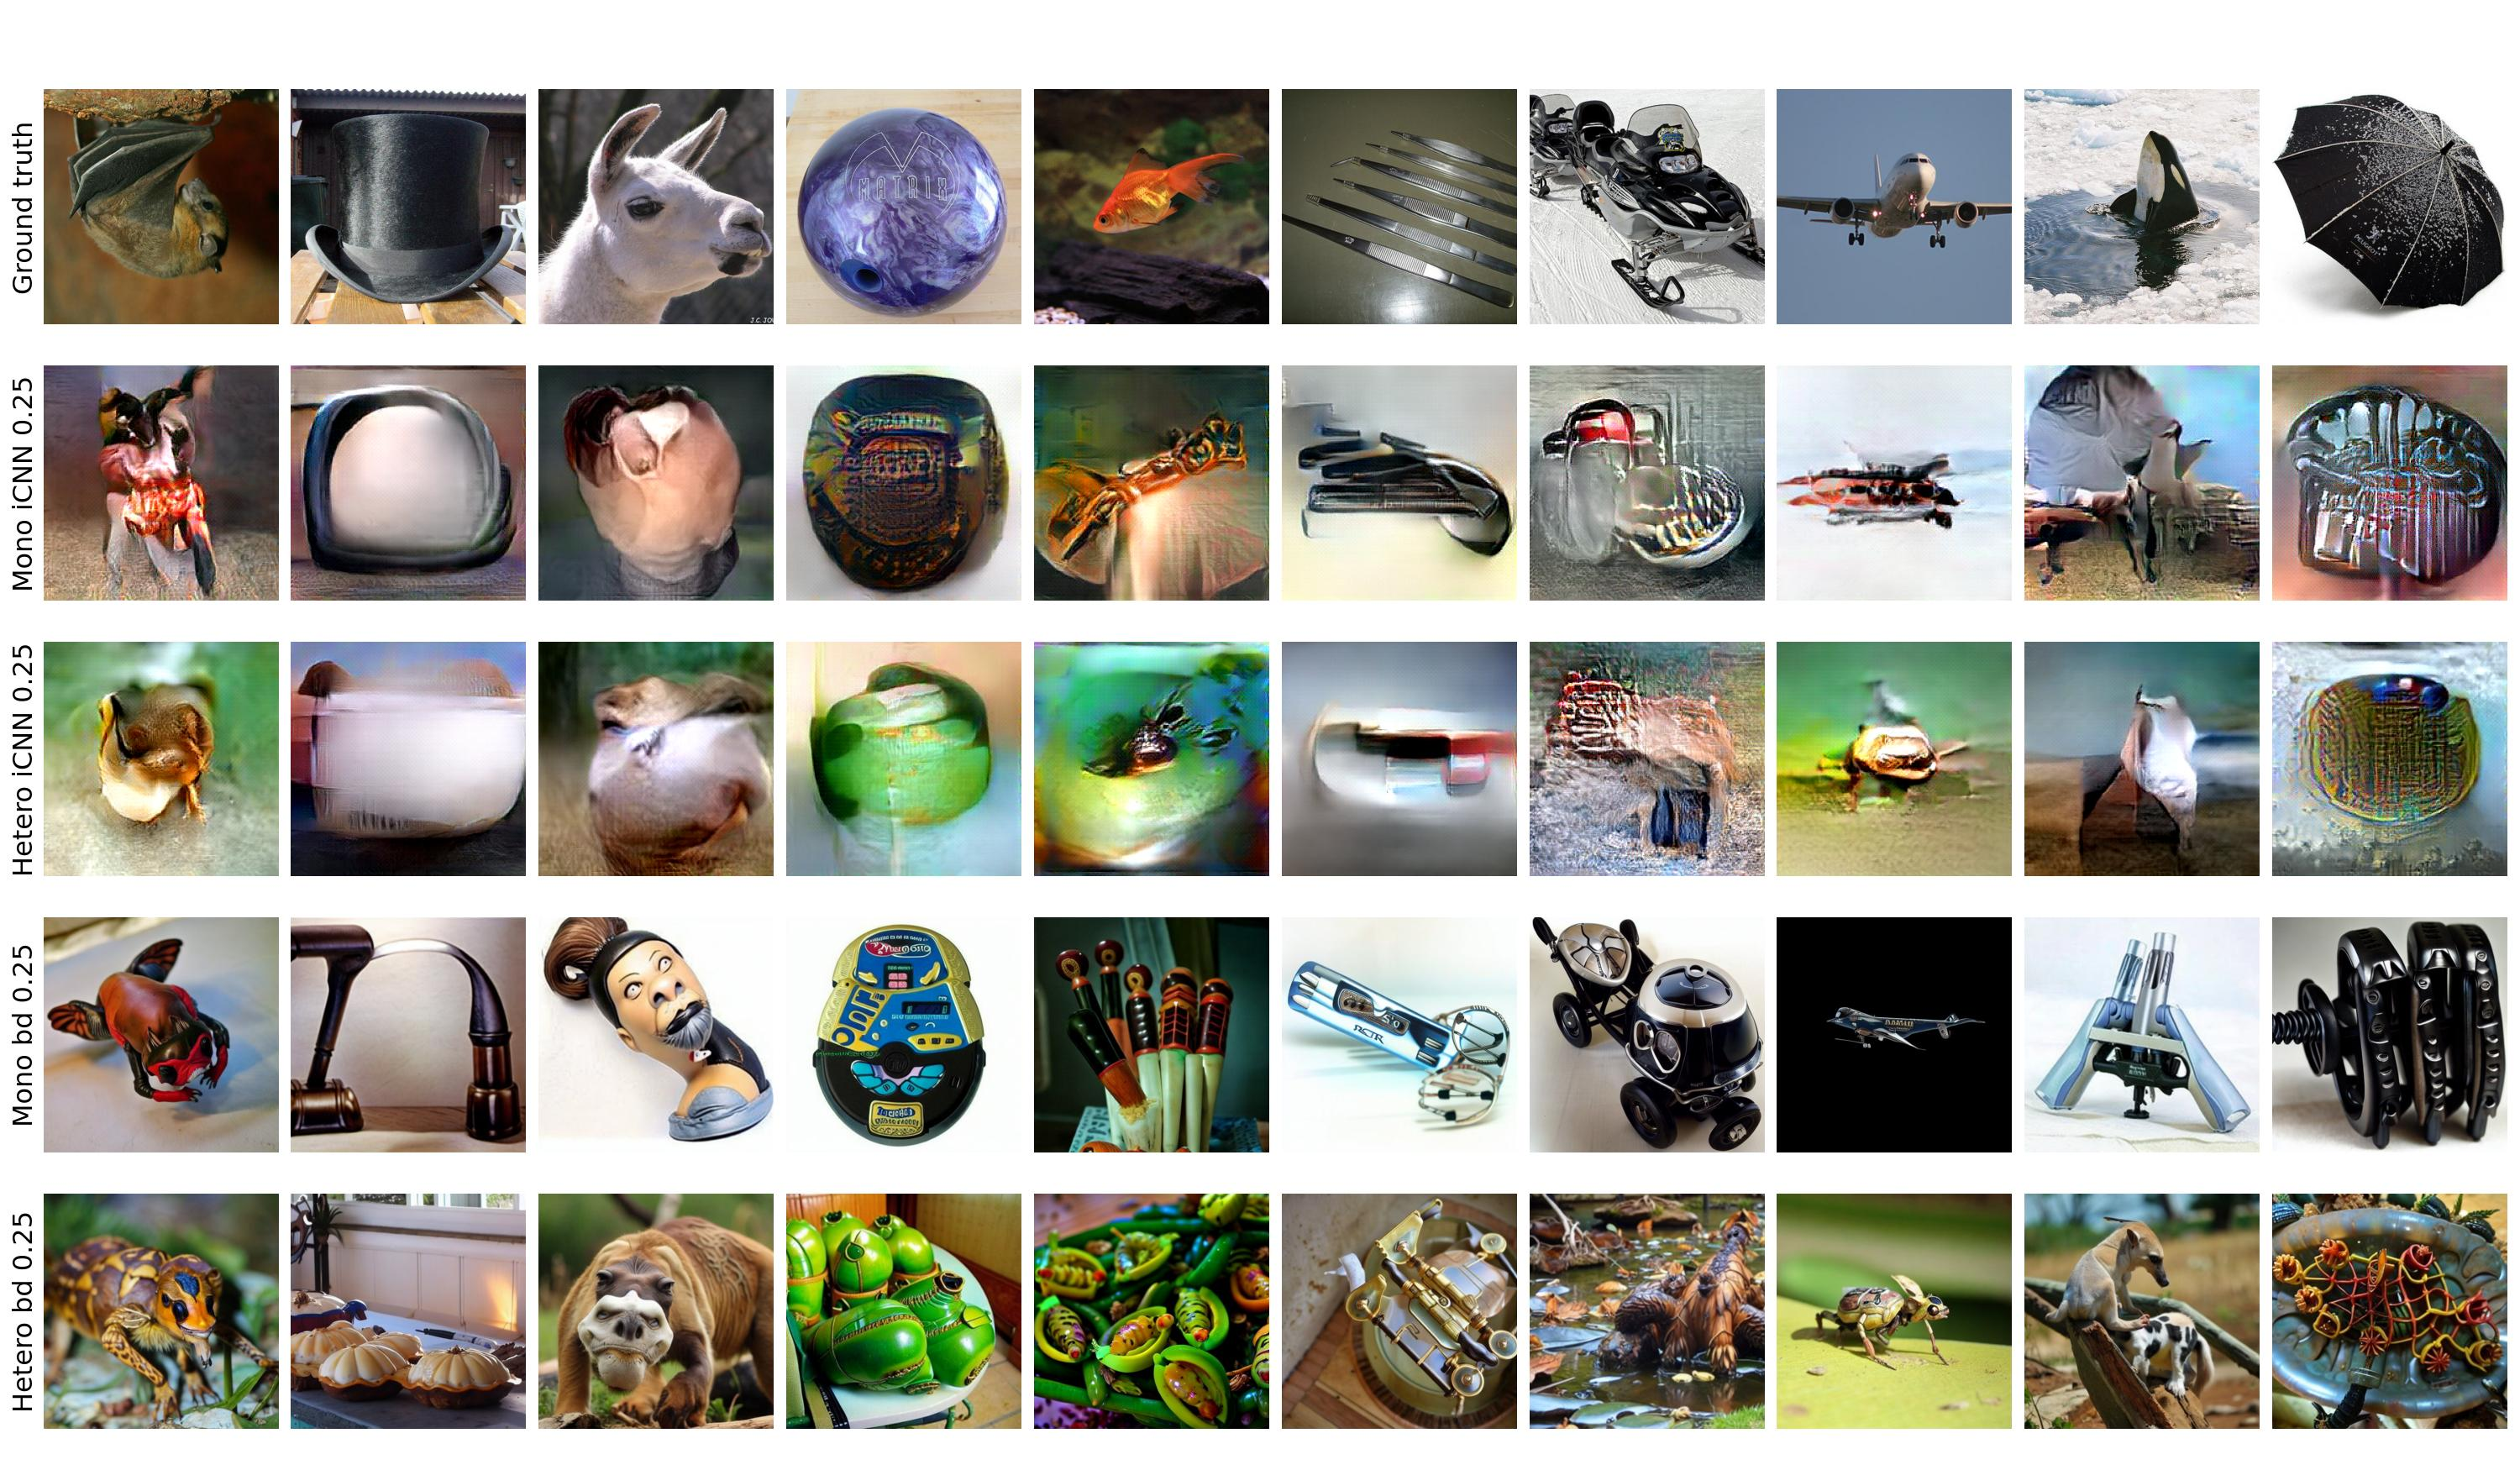
\includegraphics[width=1\textwidth]{plots/dropout_discussion_test.JPEG}
  \caption{Qualitative Results for monotone vs.\ heterogeneous training images on Natural Test Images}\label{fig:dropout_discussion_test}
\end{figure}

\subsubsection{Future Directions}

The results of the dropout experiment showed that the diversity of the training data set can have a significant influence on the decoding of brain activity and the reconstruction of images. However, the exact direction and nature of the influence on the  reconstructions is still unclear. The results of this study were inconclusive in this respect. Further research is needed on the influence of the diversity of training images on brain decoding.To this end, further different types of dropout could be used. For example, it would be possible to use dropout based on the actual semantic categories (e.g.\ using the stimulus code), so that the results do not depend on the UMAP embedding and random initial conditions during clustering. Furthermore, a more sophisticated algorithm could be used to separate the monotonous from the heterogeneous images that would also include semantic information. 

One limitation of the study is that subsampling is only possible top-down. This means that a large data set is required, which is first reduced. Ideally, there would be a way to evaluate the quality of an existing subsample iteratively from a bottom-up perspective  to determine what an image should look like that needs to be added to the dataset to improve the performance. One possibility could be an active learning approach\cite{senerActiveLearningConvolutional2018, guoDeepCoreComprehensiveLibrary2022}, which could be used during training to always look for the next image that would improve the performance. Ultimately, the aim of this study was to investigate how the nature of a dataset needs to be in order to optimise reconstruction performance. These results could then be used to create optimised training data sets that would be shown to subjects in future MRI studies. This optimised training data set does not necessarily have to consist of a sub-sample of natural images. Dataset distillation\cite{wangDatasetDistillation2018,yuDatasetDistillationComprehensive2024} could be used to create an artificial training dataset that is optimised to improve the decoders, allowing better generalisation to all possible test images. Further research is needed to determine what such an artificial training dataset might look like and whether, for example, it is necessary to show subjects natural training images at all or if it might be better to only show abstract, generated images. 



% Innerhalb meiner Bubble:
% - Man könnte den dropout noch stärker machen
% - Category based dropout could be used instead (first, find the categories in the dataset)
% - Wir sind leider nur in der Lage das Subsampling top-down durchzuführen, also wenn ein großer schöner voller Datensatz zur Verfügung steht, besser wäre ein Bottom-Up approach, bei dem kein voller Datensatz von nöten ist. Wo man quasi ohne das gesamte Datenuniversum zu kennen die Qualität (bzw. Diversität) zweier subsampled Datasets untersuchen kann. 
% - Idealerweise kriegen wir auch eine Möglichkeit hin, die Qualität eines Datensatzes im vorhinein bottom-up zu bestimmen. Also nicht so einen top-down subsampling approach zu fahren (man muss eine Gesamtmenge an Bildern haben), sondern eine Möglicheit hat top-down nach Bildern zu suchen, die das current subsample so gut wie möglich verbessern würden
  % - Top down wäre eine Metrik sehr cool, die bestimmen könnte, wie gut ein Datensatz ist in der Reconstruction, bevor man ihn für den tatsächlichen Versuch benutzen würde.

% Mit anderer Literatur
% - In dem review \cite{guoDeepCoreComprehensiveLibrary2022} Werden unterschiedliche Coreset Selection Methods vorgestellt
  % - Wir könnten auch wie \cite{senerActiveLearningConvolutional2018} einen active learning approach probieren, der beim training vom decoder versucht jeweils immer die Bilder rauszusuchen, die den größten Effekt haben und dadurch ein ideales subsample aufbauen
% - Man könnte auch weniger Cluster machen und dafür eins pro Cluster wählen, hat aber funkttioniert, also warum sollte ich.
% - Data Distillation ist eine Möglichkeit um ein komplett neuen Datensatz zu erzeugen. 
%   - Data Distillation Definition \cite{wangDatasetDistillation2018}
%   - Dataset distillation Review \cite{yuDatasetDistillationComprehensive2024}


In summary, this experiment showed that diversity-based subsampling has an impact on reconstruction performance, but that this impact needs further investigation in terms of direction and exact magnitude. In particular, the brain diffuser algorithm performed very poorly with the artificial shapes, and its decoder performance improved only marginally even with a larger amount of training data (see the random dropout results). The following results therefore look for ways to improve the performance of the brain diffuser, especially with artificial shapes.

% Überleitung zu den nächsten Experimenten (in zusammenfassender Form, die Überleitung selbst ist am Anfang des nächsten Chapters)
% - Brain-diffser hat Probleme
%   - Clipvision hat große Probleme bei den artificial Shapes überhaupt etwas zu lernen (siehe z.B. die Ergebnisse bei den random translatorn)
%   - Auch Cliptext ist dort nicht besonders gut. 
%   - Also versuchen wir im Folgenden genau an diesen beiden Stellschrauben was zu verändern um die Ergebnisse hier besser zu machen. 
